% Beamer Presentation and Lecture Note Template
% Version 0.1
% by Paul Vesey

\mode<presentation> {
\usetheme{Antibes}
\setbeamercovered{invisible}
\setbeamertemplate{footline}[frame number]
\setbeamertemplate{navigation symbols}{} 
}

\usepackage{eurosym}
\usepackage{graphicx}
\usepackage{wasysym}
\usepackage{hyperref}
\usepackage{amsmath}
\usepackage{amssymb}
\usepackage{mathtools}
\usepackage{tikz}
\usepackage{pgf}
\usepackage{pgfplots}
\usepackage{pxfonts}
\usepackage{textcomp}
\usepackage{verbatim}
\usepackage{color}
\usepackage{xcolor}
\usepackage{fix-cm}


\author{Sara-Jane Kickham}
\institute[LIT]
{
Limerick Institute of Technology \\
\medskip
{\emph{sara-jane.kickham@lit.ie}}
}
\date{2017-2018}



%\usepackage{bm} 
% For typesetting bold math (not \mathbold)
%\logo{\includegraphics[height=0.6cm]{yourlogo.eps}}
%
\title[Introduction to Project Management]{Introduction to Project Management}


\begin{document}
%
\usetikzlibrary{arrows}
\usepgflibrary{patterns}



\thispagestyle{empty} % Remove page numbering on this page

%----------------------------------------------------------------------------------------
%	TITLE SECTION
%----------------------------------------------------------------------------------------

\hrule

\vspace*{0.7cm} % Space between the start of the title and the top of the grey box


\begin{flushright}
\Huge Event Project Management \\
\vspace*{0.7cm}
\Large BA (Hons) in Business Studies with Event Management\\
Year 4 (2017-2018)
\end{flushright}

\vspace*{0.7cm} % Space between the end of the title and the bottom of the grey box
	
\normalsize

\hrule

%----------------------------------------------------------------------------------------

\vfill % Space between the title box and author information

%----------------------------------------------------------------------------------------
%	AUTHOR NAME AND INFORMATION SECTION
%----------------------------------------------------------------------------------------

{\centering \large 
\hfill Sara-Jane Kickham, \scriptsize BA(Hons), MSc\normalsize \\
\hfill Limerick Institute of Technology \\
\hfill Department of Food \& Tourism \\
\vspace*{0.7cm} 
\hrule} % Horizontal line, thickness changed here

%----------------------------------------------------------------------------------------

\clearpage % Whitespace to the end of the page

\newpage




\thispagestyle{empty}
\tableofcontents
\newpage
\section{Introduction}


\begin{frame}
\titlepage
\end{frame}\begin{center}\line(1,0){250}\end{center}
%
%
\begin{center}\line(1,0){250}\end{center}



\begin{frame}
\frametitle{What is a Project?}
A project is a temporary endeavour to create a unique product, service or result.\\
\begin{itemize}
\item Temporary: it has a start and an end
\item Unique Product, Service or Result
\item Progressive Elaboration
\end{itemize}
\end{frame}
\begin{center}\line(1,0){250}\end{center}







\begin{frame}
\frametitle{Project v. Operational Work}
Work can be categorised as either projects or operations, although there may be an overlap.\\
\textbf{Shared Characteristics:}\\
\begin{itemize}
\item Performed by people
\item Constrained by resources
\item Planned, executed and controlled
\end{itemize}
\end{frame}
\begin{center}\line(1,0){250}\end{center}



\begin{frame}
\frametitle{Project v. Operational Work}
Design of a new event site\\
Production of a play\\
Design of a concert stage\\
Construction of an event venue\\
Annual Accounts of an event company\\
\end{frame}
\begin{center}\line(1,0){250}\end{center}



\begin{frame}
\frametitle{Project v. Operational Work}
Design of a new event site -- Project\\
Production of a play -- Project \\
Design of a concert stage -- Project (overlap?)\\
Construction of an event venue -- Project (overlap?)\\
Annual Accounts of an event company -- Operations\\
\end{frame}
\begin{center}\line(1,0){250}\end{center}
Sometimes confusion can arise where an organisation makes its way by executing projects.  Consider a construction company that is constructing a new building; they do this all of the time, and may be executing numerous similar works, however each construction job remains a project.  The competitive advantage that can be leveraged by construction organisations is to streamline the processes that deliver projects.  




\begin{frame}
\frametitle{What is Project Management?}
\textit{Project Management is the application of knowledge, skills, tools and techniques to project activities to meet project requirements}.\\
\textbf{Managing Projects includes:}\\
\begin{itemize}
	\item Identifying Requirements
	\item Establishing clear \textbf{and achievable} objectives
	\item Balancing quality, scope, time and cost
	\item Adaptation of specs, plans, and approach to meet the requirements of project stakeholders
\end{itemize}
\end{frame}
\begin{center}\line(1,0){250}\end{center}




\begin{frame}
\frametitle{Project Management}
\textit{Project Management is the application of knowledge, skills, tools and techniques to project activities to meet project requirements}.\\
\textbf{Areas of Expertise:}\\
\begin{itemize}
\item Project Management Body of Knowledge
\item Application Area Knowledge, Standards and Regulations
\item Understanding the Project Environment
\item General Management knowledge and skills
\item Interpersonal Skills
\end{itemize}
\end{frame}
\begin{center}\line(1,0){250}\end{center}



\begin{frame}
\frametitle{Areas of Expertise}

 \begin{figure}
 	\centering
 		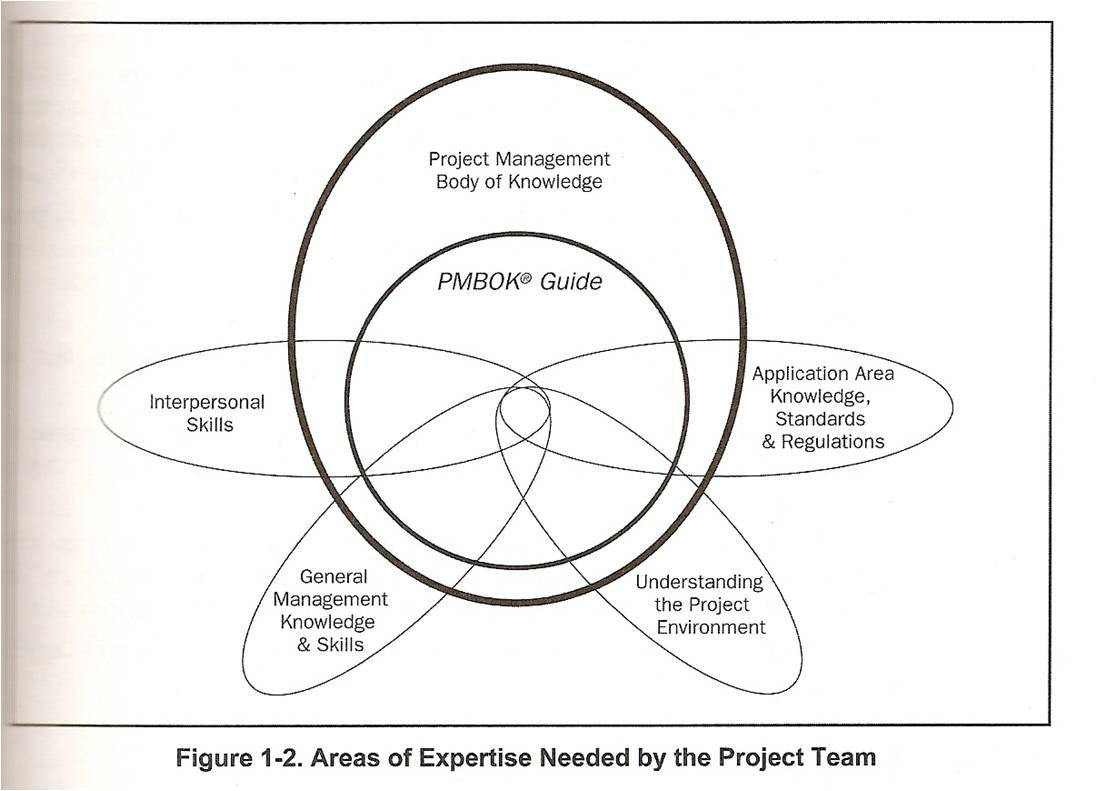
\includegraphics[width = 7cm]{images/Fig1-2old.jpg}
	\caption{Ref: Project Management Institute (2004) A Guide to the Project Management Body of Knowledge (PMBOK Guide), 3rd Edition; Project Management Institute, ISBN 978-1-930699-45-8}
 	\label{fig:1-2old}
 \end{figure}
\end{frame}
\begin{center}\line(1,0){250}\end{center}



\begin{frame}
\frametitle{Application Area Knowledge}
Functional Departments and Supporting Disciplines \\
	\begin{itemize}
	\item legal, finance, marketing, logistics
	\end{itemize}
Technical Elements \\
	\begin{itemize}
	\item Production, IT, Sound \& Light.
	\end{itemize}
Management Specialization \\
	\begin{itemize}
	\item Health \& Safety, Event Production, etc.
	\end{itemize}
Industry Groups \\
	\begin{itemize}
	\item Telecoms, Financial Services, etc.
	\end{itemize}
\end{frame}
\begin{center}\line(1,0){250}\end{center}



\begin{frame}
\frametitle{Standards \& Regulations \hfill \textit{aside}}
\textbf{Standard;} established by consensus and approved by a recognized body that provides for common and repeated use, rules, guidelines or characteristics for activities or their results aimed at the achievement of the optimum degree of order in a given context\\
\begin{itemize}
\item ANSI, ISO, BS, etc.
\end{itemize}

\textbf{Regulations;} a government imposed requirement, which specifies product, process or service characteristics, including the applicable administrative provisions, with which compliance is mandatory.\\
\begin{itemize}
\item H\&S Regs, etc. 
\end{itemize}
\end{frame}
\begin{center}\line(1,0){250}\end{center}


\begin{frame}
\frametitle{Standards \& Regulations \hfill \textit{aside}}
\begin{itemize}
\item Guidelines, upon general acceptance, often become `Standards'
\item Standards (or Guidelines) often become Regulations
		\begin{itemize}
		\item QWERTY keyboard (not efficient)
		\item SI 311: Retail Petroleum Licence
		\item SI 80 of 2013 bucks this trend
		\end{itemize}
\end{itemize}
\end{frame}
\begin{center}\line(1,0){250}\end{center}



\begin{frame}
\frametitle{Project Environment}
\textbf{Cultural \& Social Environment}\\
\begin{itemize}
	\item How will the project effect people and/or how will people effect the project? \textit{Croke Park, Olympics}
\end{itemize}
\textbf{International \& Political Environment}\\
\begin{itemize}
	\item Impact of Local Legislation; Stability of political regime \textit{Do you want to organise an event in Iraq, Syria, Afghanistan?}
\end{itemize}
\textbf{Physical Environment }\\
\begin{itemize}
	\item Impact on local ecology, geography, historical sites etc. 
\end{itemize}
\end{frame}
\begin{center}\line(1,0){250}\end{center}



\begin{frame}
\frametitle{General Management Knowledge \& Skills}
\textbf{Financial Management \& Accounting}\\
\textbf{Purchasing \& Procurement}\\
\textbf{Sales \& Marketing}\\
\textbf{Contracts \& Commercial Law}\\
\textbf{Logistics \& Supply Chain}\\
\ldots 
\end{frame}
\begin{center}\line(1,0){250}\end{center}



\begin{frame}
\frametitle{Interpersonal Skills}
\textbf{Effective Communication}\\
\textbf{Influencing the Organisation}\\
\textbf{Leadership}\\
\textbf{Motivation}  \\
\begin{itemize}
	\item self and others
\end{itemize}
\textbf{Negotiation \& Conflict Management}\\
\textbf{Problem solving} \\
\begin{itemize}
	\item Skill and judgment, not just authority to make decisions 
\end{itemize}
\end{frame}
\begin{center}\line(1,0){250}\end{center}



\begin{frame}
\frametitle{Project Management Body of Knowledge (PMBOK\textregistered)}
Consists of Ten (10) Knowledge Areas
\begin{enumerate}
\item Project Integration Management
\item Project Scope Management
\item Project Time Management
\item Project Cost Management
\item Project Quality Management
\item Project Human Resource Management
\item Project Communications Management
\item Project Risk Management
\item Project Procurement Management
\item Project Stakeholder Management
\end{enumerate}
\end{frame}
\begin{center}\line(1,0){250}\end{center}





\begin{frame}
\frametitle{Project Management Context}
 \begin{figure}
 	\centering
 		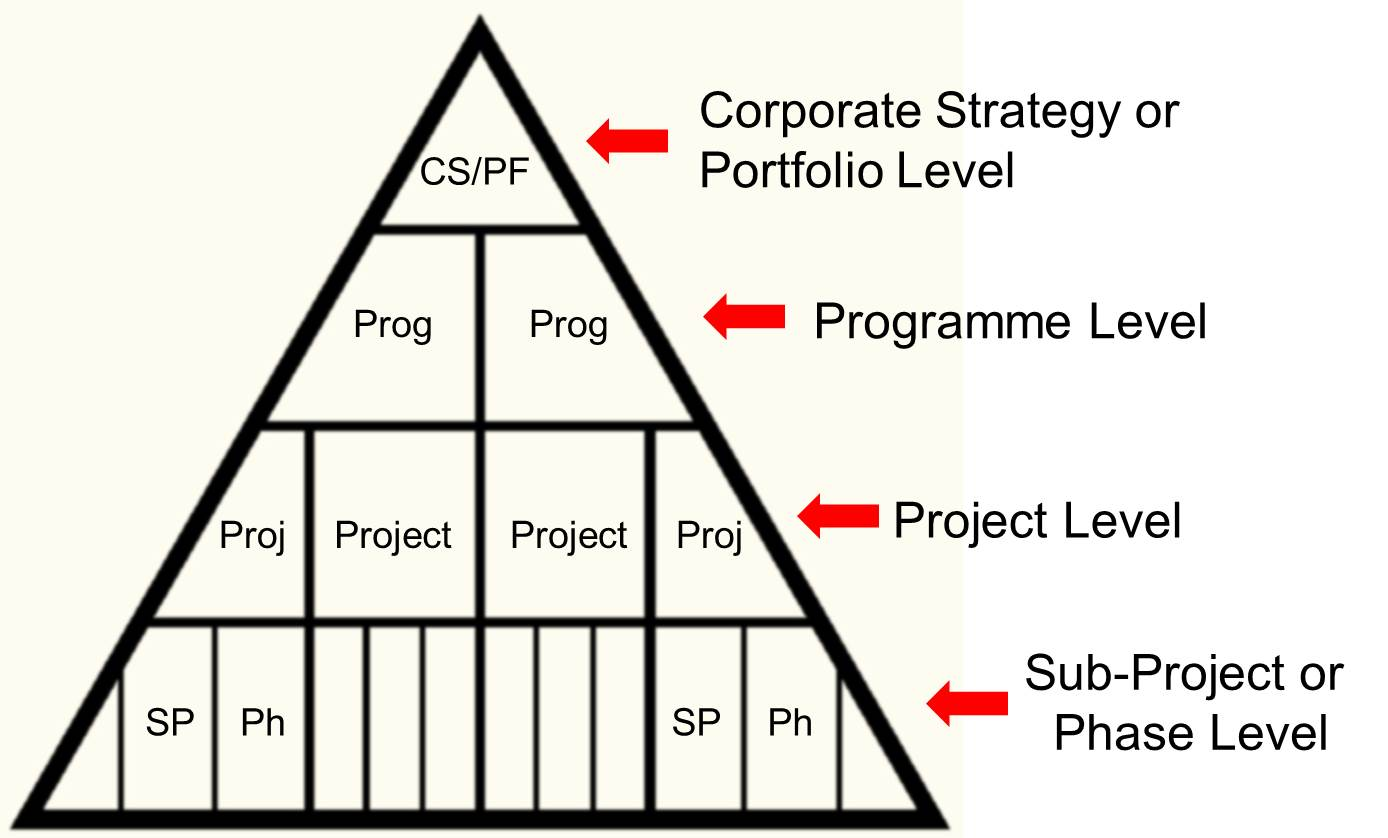
\includegraphics[width = 7cm]{images/context.jpg}
	\caption{Project Management tends to exist within a larger framework}
 	\label{fig:context}
 \end{figure}
\end{frame}
\begin{center}\line(1,0){250}\end{center}



\begin{frame}
\frametitle{Project Management Context}
\textbf{Portfolio}
\begin{itemize}
	\item Collection of Projects or Programs grouped together to facilitate effective management
\end{itemize}
\textbf{Program}
\begin{itemize}
	\item Group of related projects managed in a coordinated way in order to obtain benefits not available from managing individually
\end{itemize}
\textbf{Sub-Project}
\begin{itemize}
	\item Projects in their own right, but form part of a larger overall project.
\end{itemize}
\end{frame}
\begin{center}\line(1,0){250}\end{center}



\begin{frame}
\frametitle{Project Management Office (PMO)}
Typical of a large construction firm or MNC's\\
Not always in direct control of projects/programs\\
Often concerned with Support and/or Reporting Functions\\
\begin{itemize}
	\item Centralised Reporting
	\item Standard Policies
	\item Training
	\item Knowledge Base or Conduit to Specialist Knowledge
	\item Development of Standard Tools and Techniques
	\item Selection of Software suites...
\end{itemize}
\end{frame}
\begin{center}\line(1,0){250}\end{center}

\section{Project Life Cycle}


\begin{frame}
\frametitle{Project Life Cycle}
Any project can be broken down into several discrete phases.\\
These phases then make up the overall Project Life Cycle.\\
Knowledge of the project life cycle will give an insight into:\\
\begin{itemize}
	\item Cash flow projections
	\item Resource projections
	\item Stakeholder influence
	\item Cost of changes
	\item Etc.
\end{itemize}
NOT TO BE CONFUSED WITH A PRODUCT LIFE CYCLE\ldots\\
\end{frame}
\begin{center}\line(1,0){250}\end{center}



\begin{frame}
\frametitle{Characteristics of the Project Life Cycle}
 \begin{figure}
 	\centering
 		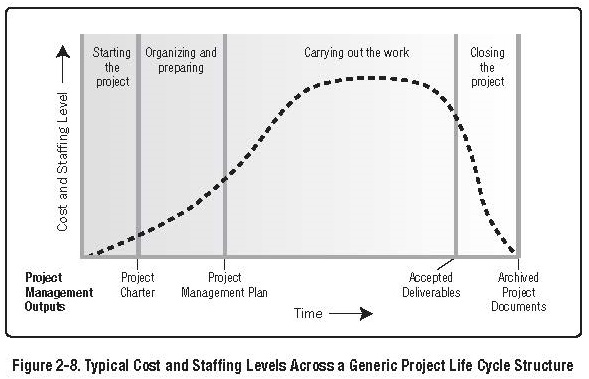
\includegraphics[width = 8cm]{images/Fig2-8.jpg}
 	\label{fig:2-8}
 \end{figure}
\end{frame}
\begin{center}\line(1,0){250}\end{center}



\begin{frame}
\frametitle{Characteristics of the Project Life Cycle}
 \begin{figure}
 	\centering
 		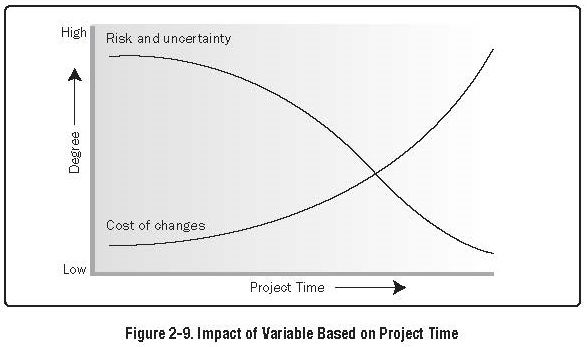
\includegraphics[width = 8cm]{images/Fig2-9.jpg}
 	\label{fig:2-9}
 \end{figure}
\end{frame}
\begin{center}\line(1,0){250}\end{center}



\begin{frame}
\frametitle{Characteristics of the Project Phases}
 \begin{figure}
 	\centering
 		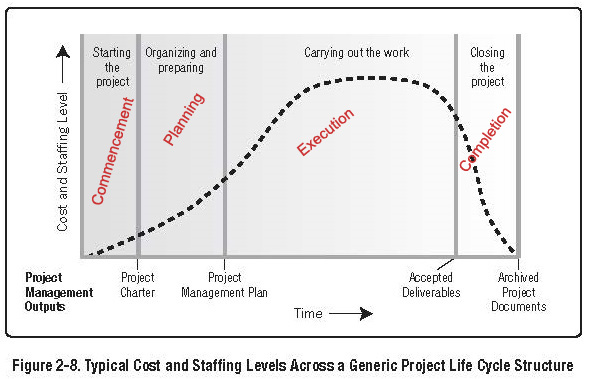
\includegraphics[width = 8cm]{images/Fig2-8edit.jpg}
 	\label{fig:2-8edit}
 \end{figure}
\end{frame}
\begin{center}\line(1,0){250}\end{center}



\begin{frame}
\frametitle{Characteristics of the Project Life Cycle}
\textbf{Phases Generally Define}\\
\begin{itemize}
	\item What technical work to undertake in each phase such as Feasibility, Design, Proposal, Execution, Handover
	\item What the deliverables are for each phase i.e Feasibility Report, Design and Specifications.
	\item Who is involved, such as Project Sponsor etc.
	\item How to Control \& Improve each phase
\end{itemize}
\end{frame}
\begin{center}\line(1,0){250}\end{center}



\begin{frame}
\frametitle{Characteristics of Project Phases}
\textbf{Phases generally:}
\begin{itemize}
	\item are sequential
	\item have specific deliverables
	\item may be sub-divided
	\item conclude with a review
		\begin{itemize}
			\item `proceed to next' or `kill point'
		\end{itemize}
	\item Can be `fast-tracked'
		\begin{itemize}
			\item Commencement of next phase before completion of preceding; carries increased risk
		\end{itemize}
	\item Formal Phase Completion does not include authorising the next phase commencement
\end{itemize}
\end{frame}
\begin{center}\line(1,0){250}\end{center}



\begin{frame}
\frametitle{Characteristics of Project Phases}
\textbf{General Comments}\\
\begin{itemize}
	\item Likelihood of Project Completion is low at the start, and increases over the life cycle; even with huge cost overruns	
		\begin{itemize}
			\item Olympics, World Cup, Limerick 2020
		\end{itemize}
	\item Decisions made early in the project life-cycle have a profound effect on project costs
	\item Costs of Change increase through the project lifecycle
	\item Phase completion and/or commencement should be controlled
\end{itemize}
\end{frame}
\begin{center}\line(1,0){250}\end{center}



\begin{frame}
\frametitle{Relevance to Project Planning}
\begin{itemize}
	\item Life Cycle Phasing not intended to `handcuff' the Project Manger\\
	\item the life-cycle phase approach provides a methodology for uniformity in project planning.\\
	\item allows for the use of standardised checklists, procedures, activities etc.\\
	\item allows for phase control - (project gates)\\
		\begin{itemize}
			\item At the end of each phase there is a meeting of the project manager, sponsor, senior management to review the phase completed, and to obtain authorisation to proceed to the next phase.
		\end{itemize}
\end{itemize}
\end{frame}
\begin{center}\line(1,0){250}\end{center}



\begin{frame}
\frametitle{Phase Control - Gating the Project}
\textbf{`end of phase' meeting'}\\
\begin{itemize}
	\item Work to date is assessed
	\item Budgets affirmed or updated
	\item Schedules affirmed or updated
	\item Decision to proceed or otherwise is made.
\end{itemize}
\textbf{Possible Decisions}\\
\begin{itemize}
	\item Proceed to next phase based on approved funding level
	\item Proceed to next with new or modified objectives
	\item Postpone approval: More information required; major budget review; etc
	\item  Terminate Project: Off-ramp, Kill Point
\end{itemize}
\end{frame}
\begin{center}\line(1,0){250}\end{center}



\begin{frame}
\frametitle{Example of Life Cycle \& Phasing}
Consider a company that has defined the following life-cycle\\
\begin{itemize}
	\item Conceptualisation
	\item Feasibility
	\item Preliminary Planning
	\item Detail Planning
	\item Execution
	\item Closure
\end{itemize}
\end{frame}
\begin{center}\line(1,0){250}\end{center}



\begin{frame}
\frametitle{Example of Life Cycle \& Phasing}
\textbf{Procedures for Conceptualisation could include:}\\
\begin{itemize}
	\item Brainstorming to identify as many solutions to a particular problem as possible
	\item Describe problem solutions in detail
\end{itemize}
\textbf{Procedures for Feasibility could include:}\\
\begin{itemize}
	\item Evaluation of all alternatives identified above
	\item Evaluation of Market Potential
	\item Evaluation of Cost Effectiveness
	\item Evaluation of Technical Issues
	\item Selection of Optimum Solution 
	\item Preparation of Project Goals and Objectives 
	\item Prepare Preliminary Cost Estimates and development Plan
\end{itemize}
\end{frame}
\begin{center}\line(1,0){250}\end{center}



\begin{frame}
\frametitle{Example of Life Cycle \& Phasing}
\textbf{Procedures for Preliminary Planning could include:}\\
\begin{itemize}
	\item Implementation of Development Plan as derived previously
	\item Completion of the Following Elements
	\begin{itemize}
		\item General Scope of Works
		\item Contractors Tasks
		\item Performance Requirements
		\item Documentation Requirements
		\item Risk Assessment
	\end{itemize}
\end{itemize}
\end{frame}
\begin{center}\line(1,0){250}\end{center}



\begin{frame}
\frametitle{Example of Life Cycle \& Phasing}
Conceptualisation \hfill$\longrightarrow\longrightarrow\longrightarrow$ Gate 1\\
Feasibility \hfill$\longrightarrow\longrightarrow\longrightarrow$ Gate 2\\
Preliminary Planning \hfill$\longrightarrow\longrightarrow\longrightarrow$ Gate 3\\
Detail Planning \hfill$\longrightarrow\longrightarrow\longrightarrow$ Gate 4\\
Execution \hfill$\longrightarrow\longrightarrow\longrightarrow$ Gate 5\\
Closure\hfill$\longrightarrow\longrightarrow\longrightarrow$ Gate 6\\
\end{frame}
\begin{center}\line(1,0){250}\end{center}




\begin{frame}
\frametitle{Decision \& Motivation Theory -  Auctions}
\textbf{English Auction}\\
\begin{itemize}
\item Open, Bids start low and increase, Highest Bidder wins, a reserve may be set.
\end{itemize}
\textbf{Dutch Auction}\\
\begin{itemize}
	\item Open, Auctioneer calls high bid and progressively lowers the bid until someone calls mine.
	\item Called Dutch because it is commonplace in the Netherlands for flower and produce auctions
	\item Dutch Auctions are considered by some as superior to English Auctions.  The buyer accepts the goods when the bid reaches a figure he/she is willing to pay.  In an English Auction, the winning bidder may get the goods at a price lower than they expected to pay.
\end{itemize}
\end{frame}
\begin{center}\line(1,0){250}\end{center}




\begin{frame}
\frametitle{The Kill Point}
Abandoning a project gets more difficult as time progresses\\
Sometimes abandoning a project is the most pragmatic business decision.\\
So why to stakeholders continue?\\
\begin{itemize}
\item \textbf{Principle of Irrational Escalation}
\item Personally invested
\item Emotion; ego; refuse to admit defeat; reputation; etc.
\item Time; cannot turn back; delivery deadline
\item Money; non-recoverable investment
\item Failure to recognise abandonment as an viable option
\end{itemize}
\end{frame}
\begin{center}\line(1,0){250}\end{center}



\section{Project Stakeholders}


\begin{frame}
\frametitle{Project Stakeholders}
Stakeholders are individuals or organisations that are actively involved in the project, or whose interests may be effected as a result of the project execution or completion. (PMBOK Defn.)\\
\begin{itemize}
	\item They may exert influence over the project
\end{itemize}
Project Management Teams must identify and manage them.
\begin{itemize}
	\item Cannot ignore them 
\end{itemize}
\end{frame}
\begin{center}\line(1,0){250}\end{center}



\begin{frame}
\frametitle{Project Stakeholders}
Stakeholders have varying levels of responsibility, authority, and input.\\
These levels can change over the course of the project\\
\begin{itemize}
	\item General Population can exert a great influence during the planning stage (Croke Park Local Residents)
	\item Influence of Population greatly diminished once planning is obtained, however may disrupt progress on other issues, such as noise, dust, traffic etc.
\end{itemize}
\end{frame}
\begin{center}\line(1,0){250}\end{center}



\begin{frame}
\frametitle{Project Stakeholders}
Stakeholders are not always easy to identify\\
Failure to Identify Key Stakeholders can have a serious negative effect on a project\\
Stakeholders can have a \textbf{negative} or \textbf{positive} effect on the project\\
\begin{itemize}
	\item \textbf{Positive Stakeholders} are those who will benefit from the successful outcome of the project
	\begin{itemize}
		\item Usually easy to identify
	\end{itemize}
	\item \textbf{Negative Stakeholders} are those who will see negative outcomes from the projects success.
	\begin{itemize}
		\item A New Hotel Project will have a negative effect on the trade of nearby hotels
		\item A new factory may have negative effect on an existing factory's ability to retain workers
	\end{itemize}
\end{itemize}
\end{frame}
\begin{center}\line(1,0){250}\end{center}



\begin{frame}
\frametitle{Project Stakeholders}
\textbf{Positive Stakeholders}\\
\begin{itemize}
	\item Their interests are best served by helping the project to succeed
\end{itemize}
\textbf{Negative Stakeholders}\\
\begin{itemize}
	\item Their interests are best served by impeding project progress
\end{itemize}
Ignoring Negative Stakeholders can put an entire project at risk of failure; suspension; financial ruin; or worse.\\
\end{frame}
\begin{center}\line(1,0){250}\end{center}



\begin{frame}
\frametitle{Project Stakeholders}
Key Stakeholders on every Project include:\\
\begin{itemize}
	\item \textbf{Project manager}. The person responsible for managing the project. 
	\item \textbf{Customer/user}. The person or organization that will use the project's product or service. There may be multiple layers of customers. For example, the customers for a new pharmaceutical product can include the doctors who prescribe it, the patients who take it and the insurers who pay for it.
	\item \textbf{Performing organization}. The enterprise whose employees are most directly involved in doing the work of the project. 
	\item \textbf{Project team members.} The group that is performing the work of the project. 
\end{itemize}
\end{frame}
\begin{center}\line(1,0){250}\end{center}


\begin{frame}
\frametitle{Project Stakeholders}
Key Stakeholders on every Project include:\\
\begin{itemize}
	\item \textbf{Project management team.} The members of the project team who are directly involved in project management activities. 
	\item \textbf{Sponsor or Funders.} The person or group that provides the financial resources, in cash or in kind, for the project. 
	\item \textbf{Influencers.} People or groups that are not directly related to the acquisition or use of the project's product, but due to an individual's position in the customer organization or performing organization, can influence, positively or negatively, the course of the project. 
	\item \textbf{PMO.} If it exists in the performing organization, the PMO can be a stakeholder if it has direct or indirect responsibility for the outcome of the project. 
\end{itemize}
\end{frame}
\begin{center}\line(1,0){250}\end{center}





\begin{frame}
\frametitle{Project Stakeholders}
\textbf{Stakeholders can be further categorized into:}\\
	\begin{itemize}
	\item Internal
	\item External
	\item Owners
	\item Investors
	\item Sellers
	\item Contractors
	\item Government agencies
	\item Lobbying organisations
	\end{itemize}
\textbf{Stakeholders roles can overlap}\\
	\begin{itemize}
	\item Construction of new fabrication unit for a factory
	\item Self Financed (Sponsor); End User; PM Team Members etc.
	\end{itemize}
\end{frame}
\begin{center}\line(1,0){250}\end{center}



\begin{frame}
\frametitle{Project Stakeholders}
Project Managers must manage stakeholders; \\
\begin{itemize}
	\item This is not an easy task as often stakeholders interests oppose each other.
\end{itemize}
Example: Wind Farms:\\
	\begin{itemize}
		\item Most people when asked say they agree that wind farms are necessary; green energy etc.
		\item Traditionally it was very difficult to obtain PP from local authorities. Legislation had to be enacted to change this. \href{http://www1.pleanala.ie/REP/200/R200723.DOC}{Kerry CC, Slaheny Energy Ltd., March 2003}
	\end{itemize}

\end{frame}
\begin{center}\line(1,0){250}\end{center}



\begin{frame}
\frametitle{Responsibility of a Project Manager to Stakeholders}
Rooted in Ethics and Ethical Behaviour\\
\begin{itemize}
\item Truthful representation of all information
\item Full disclosure of all information
\item Protection of company-proprietary information
\item Responsibility to report violations
\item Full disclosure, and in a timely manner of all conflicts of interest
\item Ensure that all PM team members comply with the above
\end{itemize}
\textbf{Ethical Behaviour may be either voluntary, or imposed by Company Policy}.\\
\end{frame}
\begin{center}\line(1,0){250}\end{center}
Many Organisation are now implementing CSR, or Corporate Social Responsibility policies.  It is thought that CSR will assist businesses to grow and mature.  There are however numerous examples of companies flouting their own CSR policies when put under pressure.




\begin{frame}
\frametitle{Managing Stakeholders}
\begin{itemize}
	\item Generally, External Stakeholders are not managed by the PMO.  PMO's tend to manage internal stakeholders, to a small degree
	\item Responsibility for Managing Stakeholders rests firmly with the Project Management Team; and the PM Team stand to lose the most if it is not effective
	\item Primary Requirement is Open Communications and Managed Expectations
\end{itemize}
\end{frame}
\begin{center}\line(1,0){250}\end{center}



\begin{frame}
\frametitle{Managing Stakeholders}
Managing Expectations:\\
\begin{itemize}
	\item \textbf{Always} build Contingency into your plans
		\begin{itemize}
			\item Be ready to offer alternatives/options that continue to meet project objectives
		\end{itemize}
	\item \textbf{Never} offer an alternative or bow to stakeholder pressure unless you are sure that your (or their) alternative will work
			\begin{itemize}
			\item Request time to evaluate alternatives
			\item If you don't, you run the very real risk of signing up to `mission impossible' and causing real damage to the trust between parties
			\end{itemize}
	\item \textbf{Beware} of modifying yours, or others, estimates on time/cost/complexity etc.
		\begin{itemize}
		\item Estimates are often used as the first point of attack on a plan. i.e. `You are too conservative here; you can shave a week off that \ldots.'
		\end{itemize} 
\end{itemize}
\end{frame}
\begin{center}\line(1,0){250}\end{center}
Project Managers are in a very strong position when it comes to managing expectations.  For the most part, stakeholder expectations are guided by what PM's have told them in meetings and reports and other communications.  However, constantly trying to please or appease stakeholders generally back-fires.  


\begin{frame}
\frametitle{Managing Stakeholders}
Managing Expectations\\
\begin{itemize}
	\item Keep it Civilised; keep emotion out of it, and don't take it personally.
	\item If you hear comments like `\textit{do what I say or else}' from your boss or project sponsor, then it's time to update your CV
		\begin{itemize}
			\item You could end up with a project that is out of control; better to keep your reputation intact.
		\end{itemize}
\end{itemize}
\end{frame}
\begin{center}\line(1,0){250}\end{center}
The Irish construction is very small, and people talk.  Associations with failed projects can have a long term effect on your career.  For the most part, this only effects those at on and above the mid management levels.  Those lower on the totem pole tend to survive better.




\begin{frame}
\frametitle{Managing Stakeholders}
\textbf{Giving Commitments}\\
At some point you have to give a commitment, \textbf{so}\dots
\begin{itemize}
\item Never commit [to a deadline] too early
\item Make sure you know what the customer is \textbf{expecting}; this is normally based on what you have led them to believe
\item Know what elements on your project have no \textbf{margin for error}, and make sure that nothing goes wrong with them.
\item When giving a commitment, make sure that you can \textbf{at least meet it}, and hopefully exceed it.
\item If you are going to fail to meet a commitment, make sure you have a \textbf{fallback} position.
\end{itemize}
\end{frame}
\begin{center}\line(1,0){250}\end{center}
Anyone with any experience of projects knows that it is not a question of 'if' something will go wrong, it's just a matter of 'when'.  The real issue is how you deal with problems when they arise.  The best PM's will either have a solution or be working on one.  In other words they are managing the situation.


\begin{frame}
\frametitle{Project Stakeholders}
 \begin{figure}
 	\centering
 		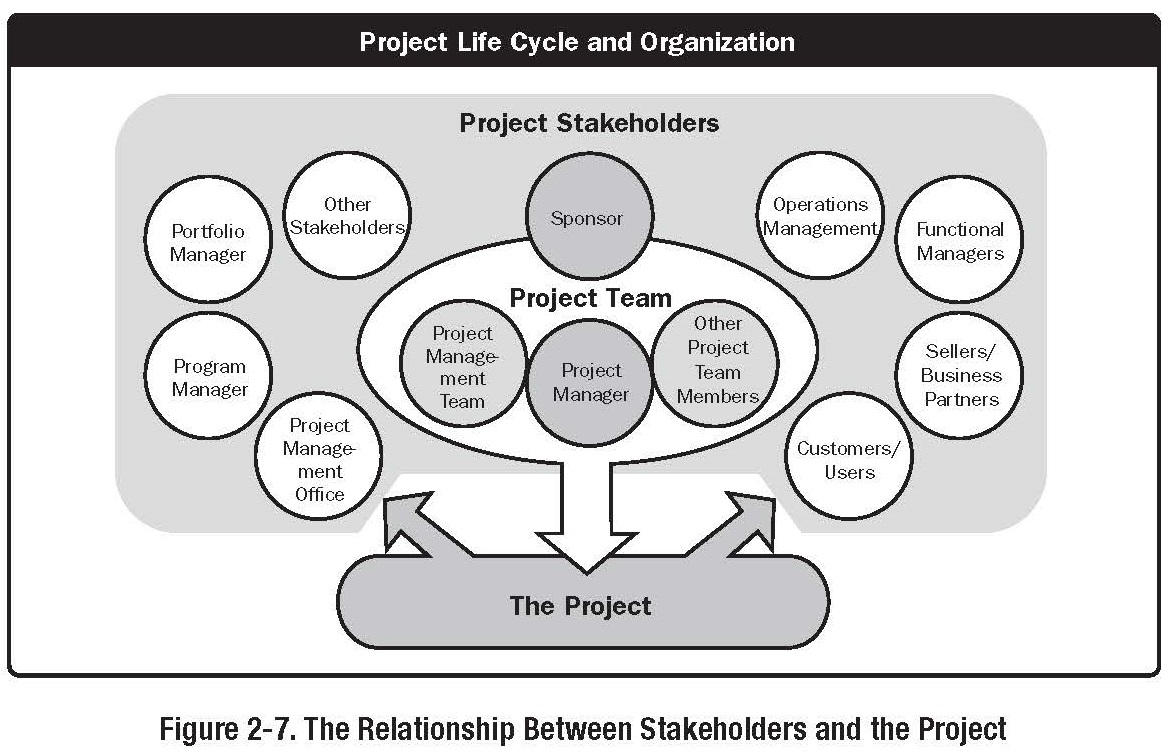
\includegraphics[width = 10cm]{images/Fig2-7.jpg}
 	\label{fig:2-7}
 \end{figure}
\end{frame}
\begin{center}\line(1,0){250}\end{center}






\section{Project Organization}


\begin{frame}
\frametitle{Project Organization}
 \begin{figure}
 	\centering
 		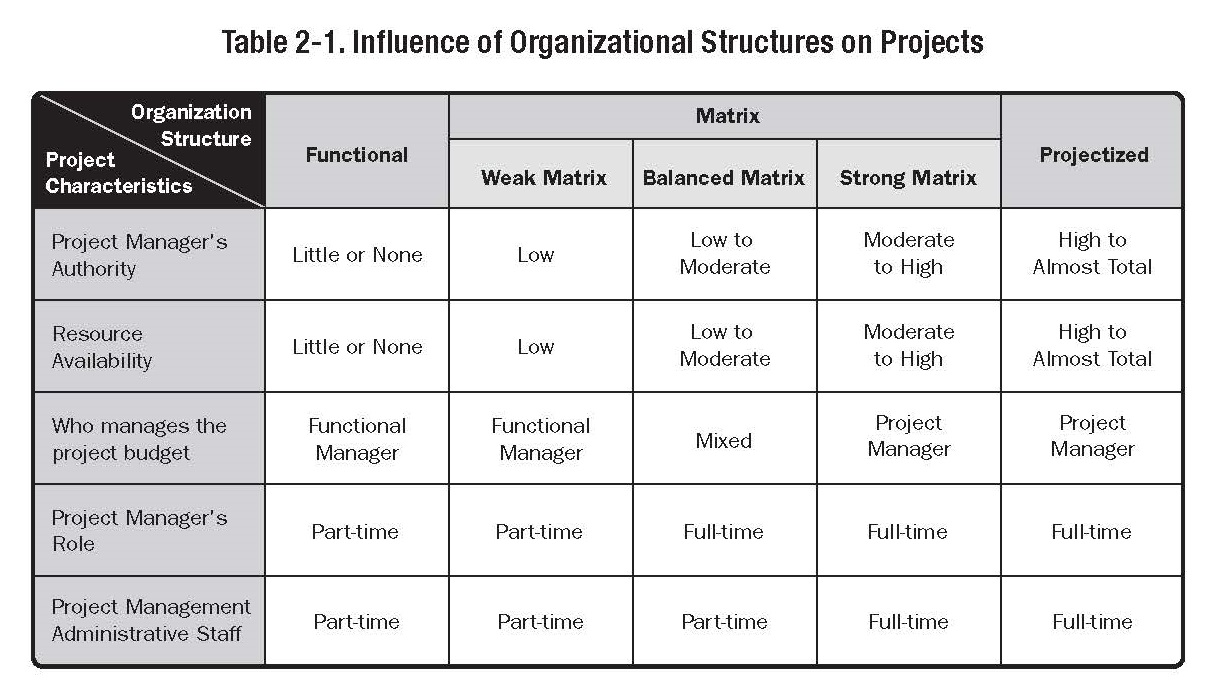
\includegraphics[width = 8cm]{images/tbl2-1.jpg}
 	\label{tbl:2-1}
 \end{figure}
\end{frame}
\begin{center}\line(1,0){250}\end{center}



\begin{frame}
\frametitle{Organisational Influences}
Projects are typically part of an organisation that is larger than the project\\
\begin{itemize}
	\item Promoter is bigger than a new festival
\end{itemize}
The maturity of an organisations Project Management Systems can (and normally does) influence the project\\
\begin{itemize}
	\item MCD have huge experience in delivering events
\end{itemize}
Key Aspects of these orgainsations are their:\\
	\begin{itemize}
		\item Organisational Systems
		\item Organisational Cultures and Styles
		\item Organisational Structures
	\end{itemize}
\end{frame}
\begin{center}\line(1,0){250}\end{center}



\begin{frame}
\frametitle{Organisational Systems}
Organisational Systems can be:\\
\begin{itemize}
\item Financial Systems
\item Reporting Systems
\item Procurement Systems
\item IT Systems
\item Communications Systems
\item Departments
\end{itemize}
In basic terms, the organisational infrastructure required to support projects\\
\begin{itemize}
\item PMBOK\textsuperscript{\textregistered} refers to many of these as \textbf{Organisational Process Assets}\
\end{itemize}\
\end{frame}
\begin{center}\line(1,0){250}\end{center}



\begin{frame}
\frametitle{Organisational Systems}
Project-based organisations are those whose operations consist primarily of projects\\
\textbf{Two categories:}\\
\begin{itemize}
	\item Organisations that derive their revenue primarily from performing projects for others under contract
	\item Organisations that have adopted Management by Projects
\end{itemize}
Non-Project based organisations often lack the management systems to support projects effectively.\\
\end{frame}
\begin{center}\line(1,0){250}\end{center}



\begin{frame}
\frametitle{Organisation Cultures and Styles}
\textbf{Cultures and Styles can be}\\
		\begin{itemize}
			\item Shared Values, norms, beliefs and expectations
			\item Policies and Procedures
			\item View of Authority Relationships
			\item Work ethic and work hours
		\end{itemize}
Such as:\\
\begin{itemize}
	\item Entrepreneurial Leadership: More likely to take on high risk project
	\item Bureaucratic Style: Less likely to take on risk
	\item Participative Style: Assists in project communications and ultimately project sucess
\end{itemize}
\end{frame}
\begin{center}\line(1,0){250}\end{center}



\begin{frame}
\frametitle{Organisational Structure}
 \begin{figure}
 	\centering
 		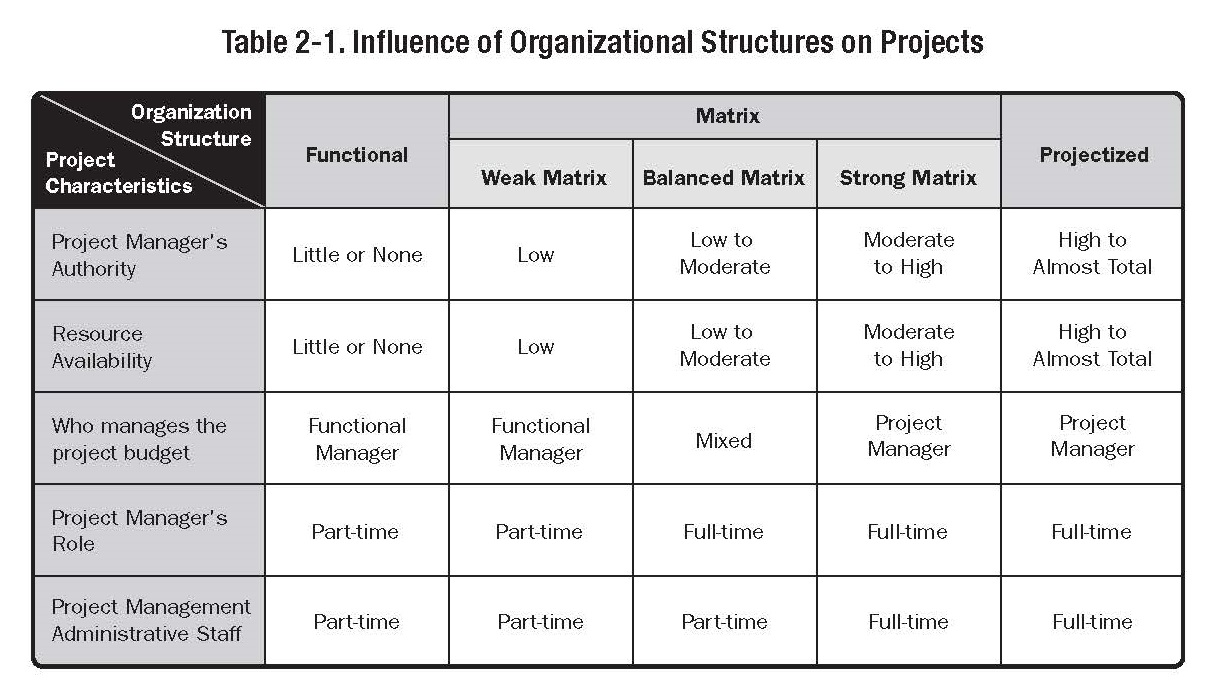
\includegraphics[width = 10cm]{images/tbl2-1.jpg}
 	\label{tbl:2-1b}
 \end{figure}
\end{frame}
\begin{center}\line(1,0){250}\end{center}



\begin{frame}
\frametitle{Organisational Structure}
\begin{figure}
	\centering
		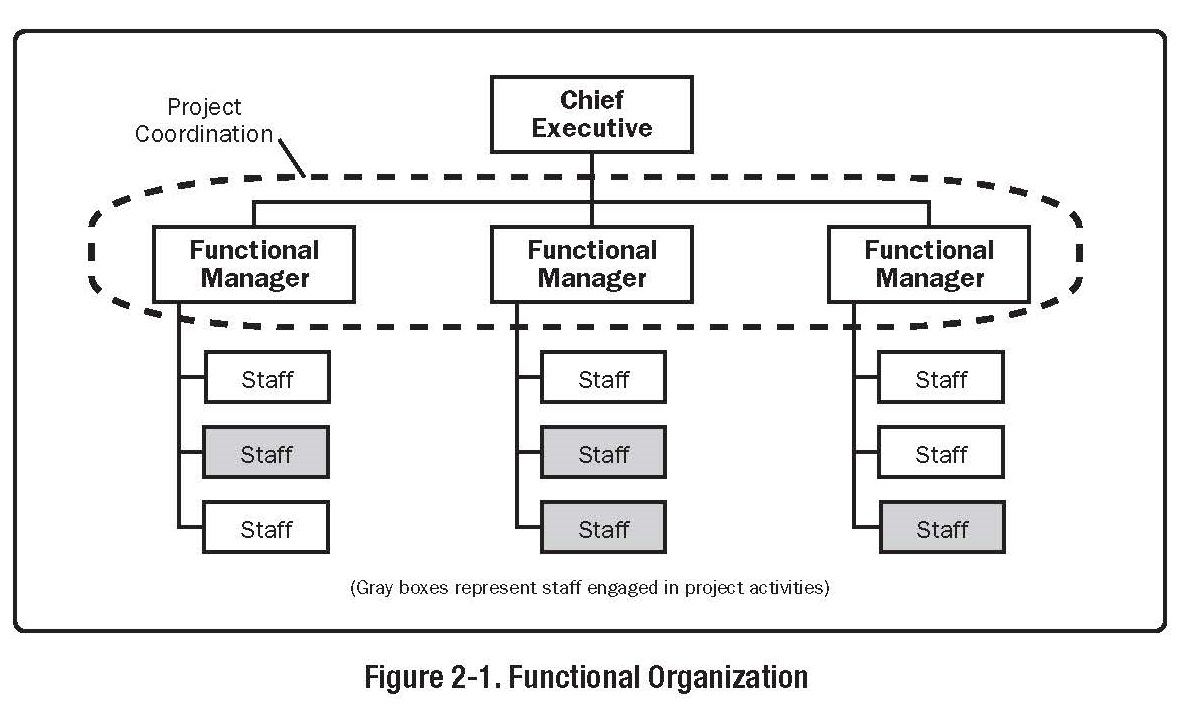
\includegraphics[width = 7cm]{images/Fig2-1.jpg}
	\label{fig:2-1}
\end{figure}Hierarchy with one clear superior\\
Staff Members grouped by functional speciality\\
Scope for Project Implementation limited\\
Project Manager has to pull from Functional Mangers\\
\end{frame}
\begin{center}\line(1,0){250}\end{center}



\begin{frame}
\frametitle{Organisational Structure}
\begin{figure}
	\centering
		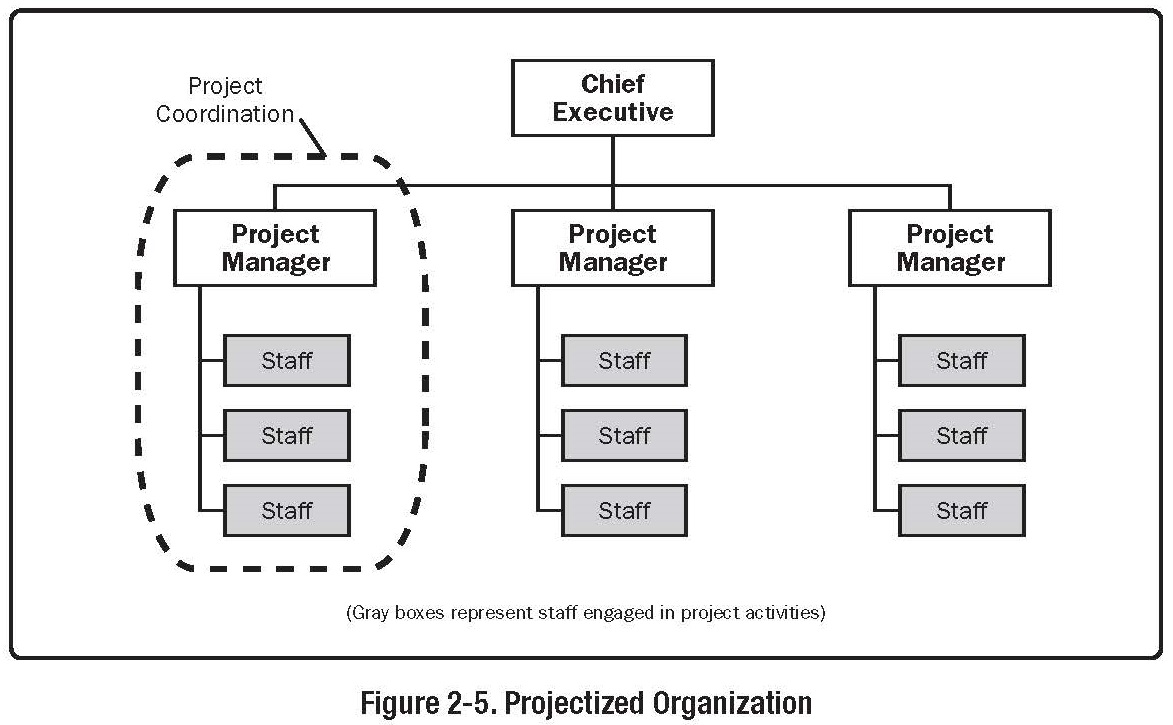
\includegraphics[width = 7cm]{images/Fig2-5.jpg}
	\label{fig:2-5}
\end{figure}Project Manager in charge of multi-discipline team\\
Project Manger has more control, authority and autonomy\\
\end{frame}
\begin{center}\line(1,0){250}\end{center}



\begin{frame}
\frametitle{Organisational Structure}
\begin{figure}
	\centering
		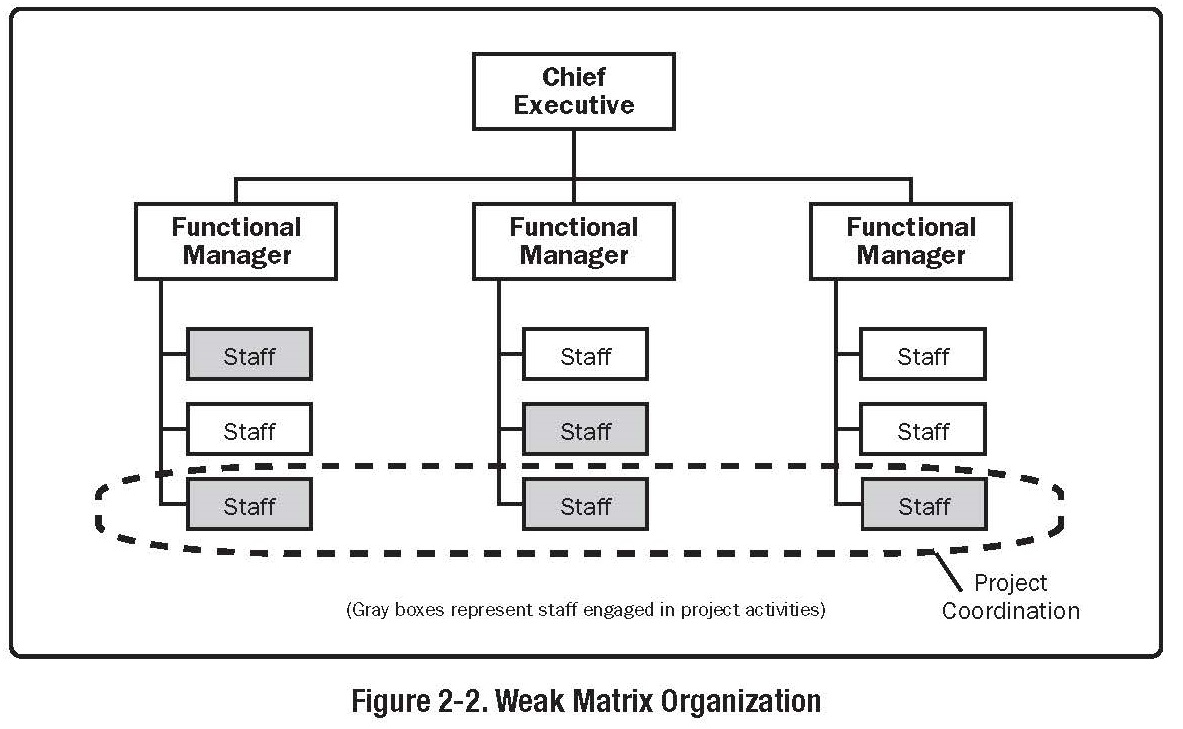
\includegraphics[width = 7cm]{images/Fig2-2.jpg}
	\label{fig:2-2}
\end{figure}Role of PM is that of coordinator and expediter\\
Little Direct Control\\
Similar to Functional organisation\\
\end{frame}
\begin{center}\line(1,0){250}\end{center}



\begin{frame}
\frametitle{Organisational Structure}
\begin{figure}
	\centering
		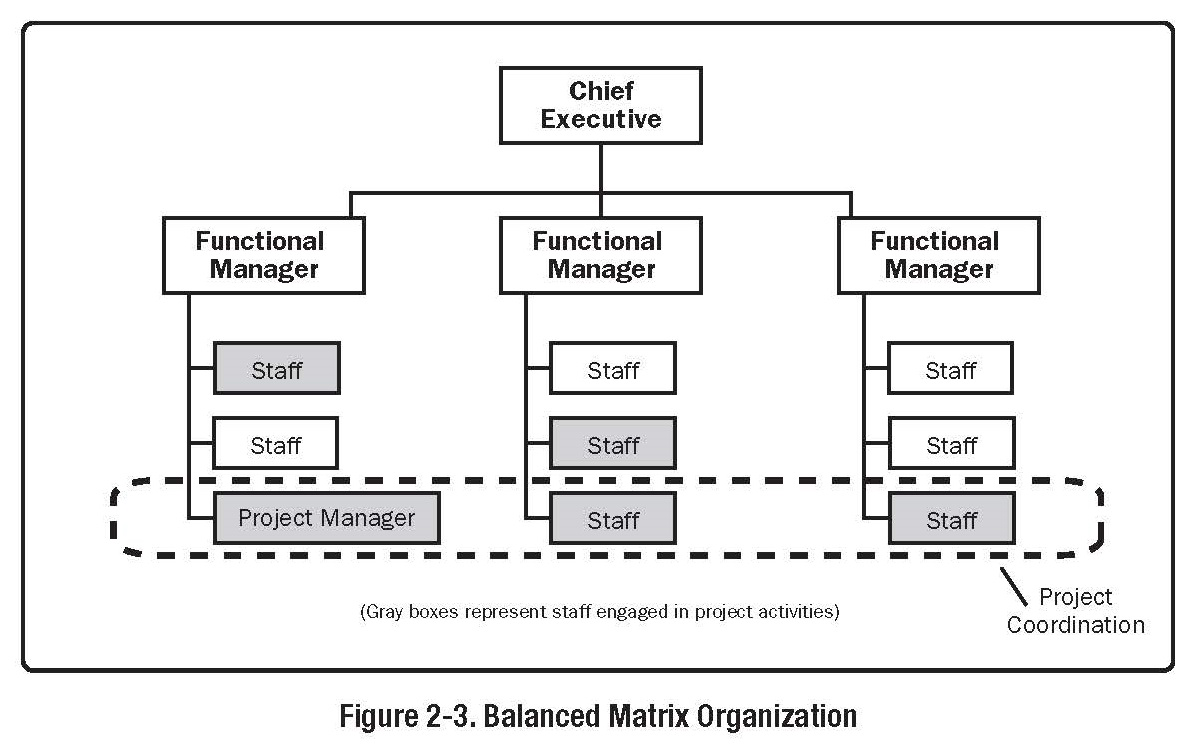
\includegraphics[width = 7cm]{images/Fig2-3.jpg}
	\label{fig:2-3}
\end{figure}PM reports to a Functional Manager\\
PM has more control, but still relies on functional Managers for resources\\
\end{frame}
\begin{center}\line(1,0){250}\end{center}



\begin{frame}
\frametitle{Organisational Structure}
\begin{figure}
	\centering
		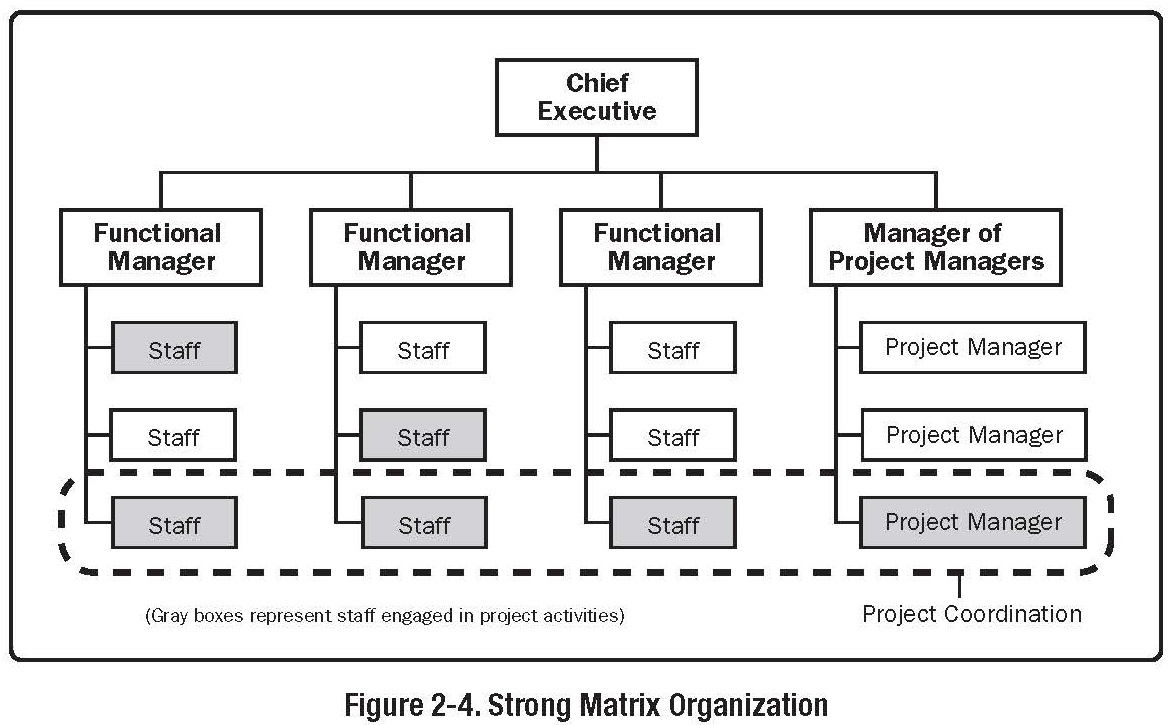
\includegraphics[width = 7cm]{images/Fig2-4.jpg}
	\label{fig:2-4}
\end{figure}PM reports to Senior PM\\
Senior PM on a better level to deal with resourcing issues\\
\end{frame}
\begin{center}\line(1,0){250}\end{center}



\begin{frame}
\frametitle{Organisational Structure}
\begin{figure}
	\centering
		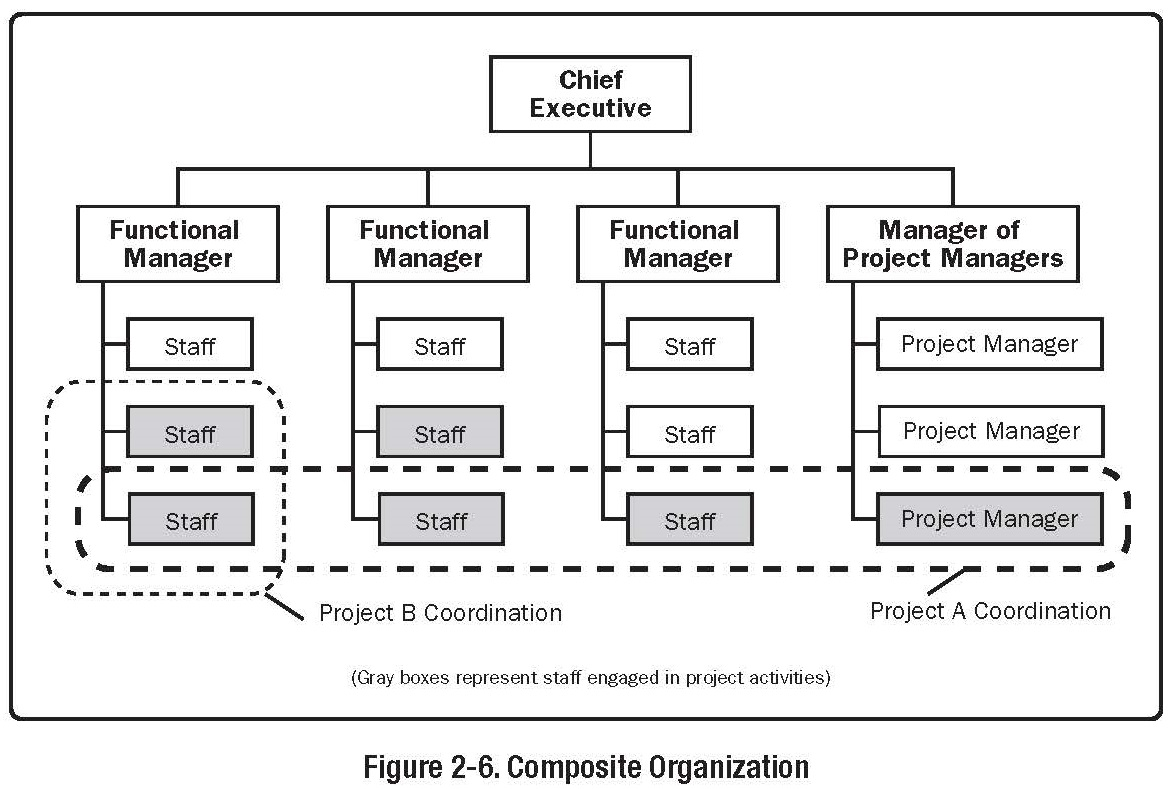
\includegraphics[width = 7cm]{images/Fig2-6.jpg}
	\label{fig:2-6}
\end{figure}Special Project Team for specific projects\\
\end{frame}
\begin{center}\line(1,0){250}\end{center}


\section{Project Management Processes}


\begin{frame}
\frametitle{Project Management}
\begin{itemize}
	\item Up to now we have been `setting the seen', i.e. looking at what a project is, who is involved, what organisation structures best support projects \& project mangers, etc.
	\item This lecture presents an overview of the project management processes used in industry.  
	\item Over the coming weeks \& months these areas are going to be presented in detail.
\end{itemize}
\end{frame}
\begin{center}\line(1,0){250}\end{center}



\begin{frame}
\frametitle{Project Management Processes}
Project Management is accomplished through \textbf{processes}, using PM knowledge, skills, tools and techniques that:\\
\begin{itemize}
	\item Receive inputs
	\item Generate outputs
\end{itemize}
\end{frame}
\begin{center}\line(1,0){250}\end{center}



\begin{frame}
\frametitle{Project Management Processes}
\begin{itemize}
	\item In order for a project to be successful, the PM team must\\
	\item Select appropriate Processes
	\item Use a \textbf{defined} approach to adapt specifications and plans to meet project (and/or product) requirements
	\item Comply with requirements to meet stakeholders needs, wants and expectations
	\item Balance the demands of Scope, Time, Cost, Quality, Resources, and Risk.
\end{itemize}
\end{frame}
\begin{center}\line(1,0){250}\end{center}



\begin{frame}
\frametitle{Project Management Process Groups}
There are 5 process groups:
\begin{enumerate}
	\item Initiating Process Group
	\item Planning Process Group
	\item Executing Process Group
	\item Monitoring and Controlling Process Group
	\item Closing Process Group
\end{enumerate}
PROCESS GROUPS ARE NOT PROJECT PHASES\\
\end{frame}
\begin{center}\line(1,0){250}\end{center}



\begin{frame}
\frametitle{Project Management Process Groups - Overview}
 \begin{figure}
 	\centering
 		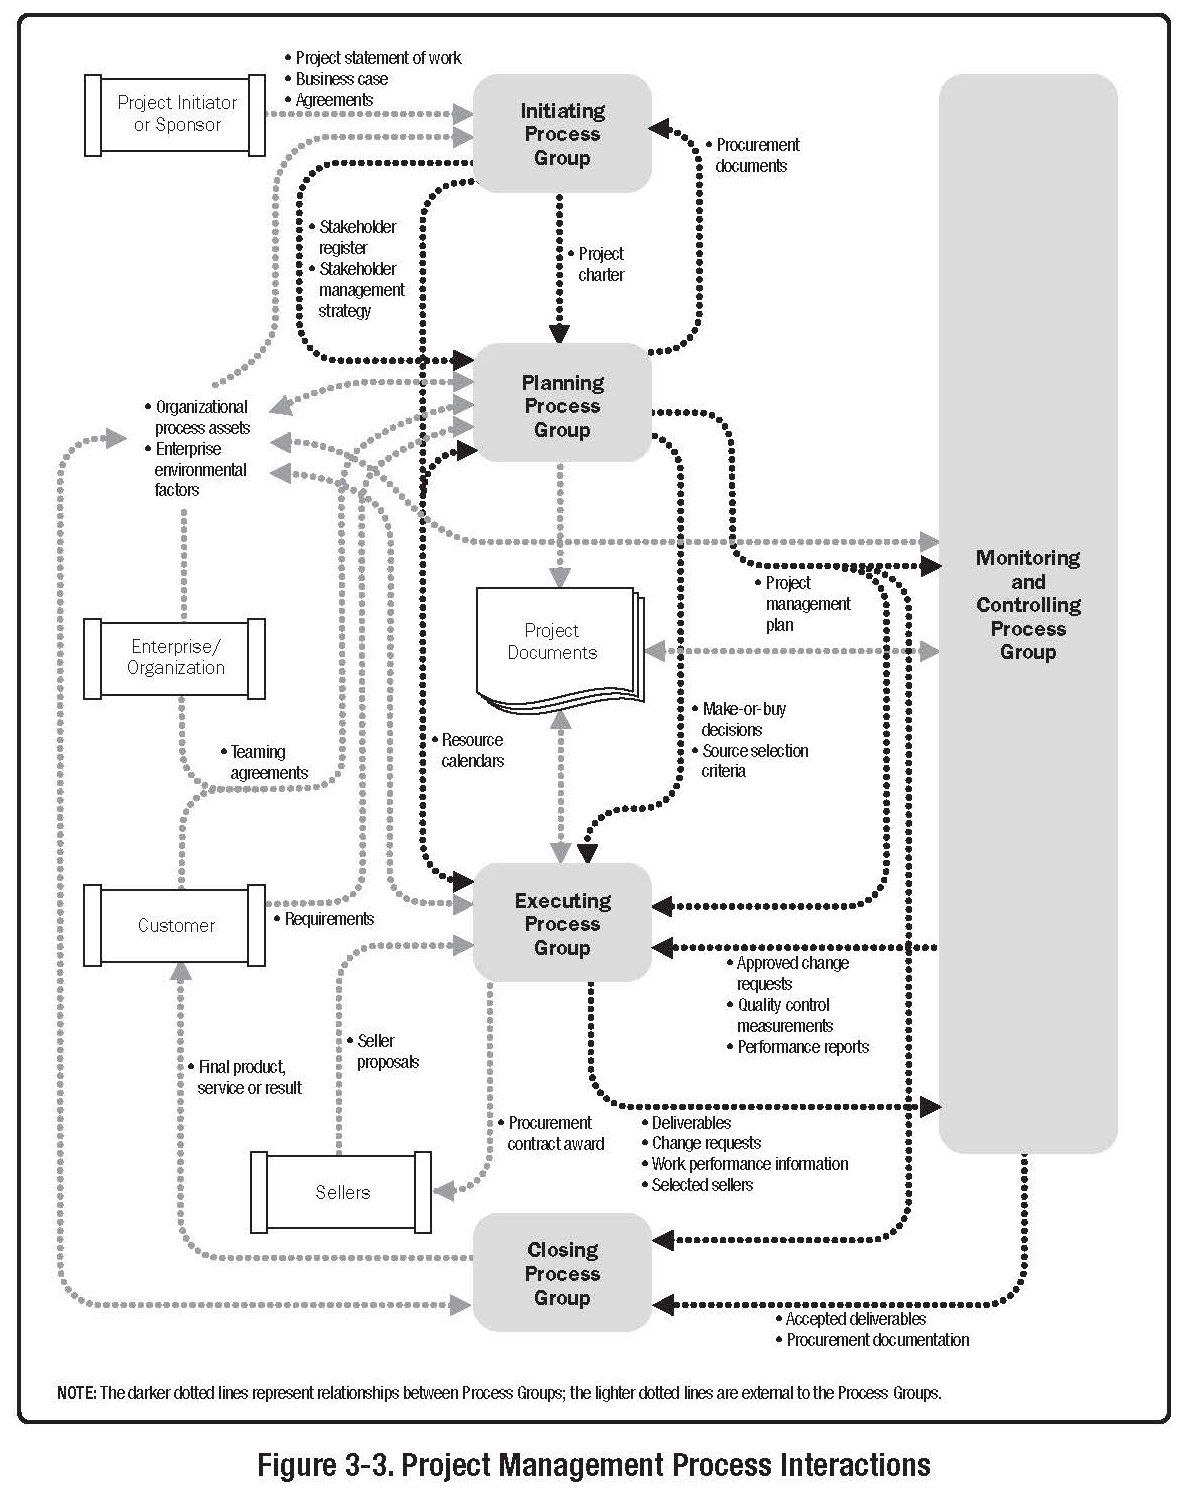
\includegraphics[width = 5cm]{images/Fig3-3.jpg}
 	\label{fig:3-3}
 \end{figure}
\end{frame}
\begin{center}\line(1,0){250}\end{center}



\begin{frame}
\frametitle{Initiating Process Group}
\begin{itemize}
	\item The Initiating Process Group Consists of the processes that facilitate the formal authorisation to start a new project or phase.\\
	\item Elements are often carried out external to the project scope of control; \\
		\begin{itemize}
			\item i.e. before embarking on a project an organisation may document its requirements, evaluate alternatives, and chose one; a project scope statement may also be generated. 
		\end{itemize}
	\item This can `blur' the boundary between the original investigation (feasibility study) and the formal initiation of the project\\
\end{itemize}
\end{frame}
\begin{center}\line(1,0){250}\end{center}



\begin{frame}
\frametitle{Initiating Process Group}
 \begin{figure}
 	\centering
 		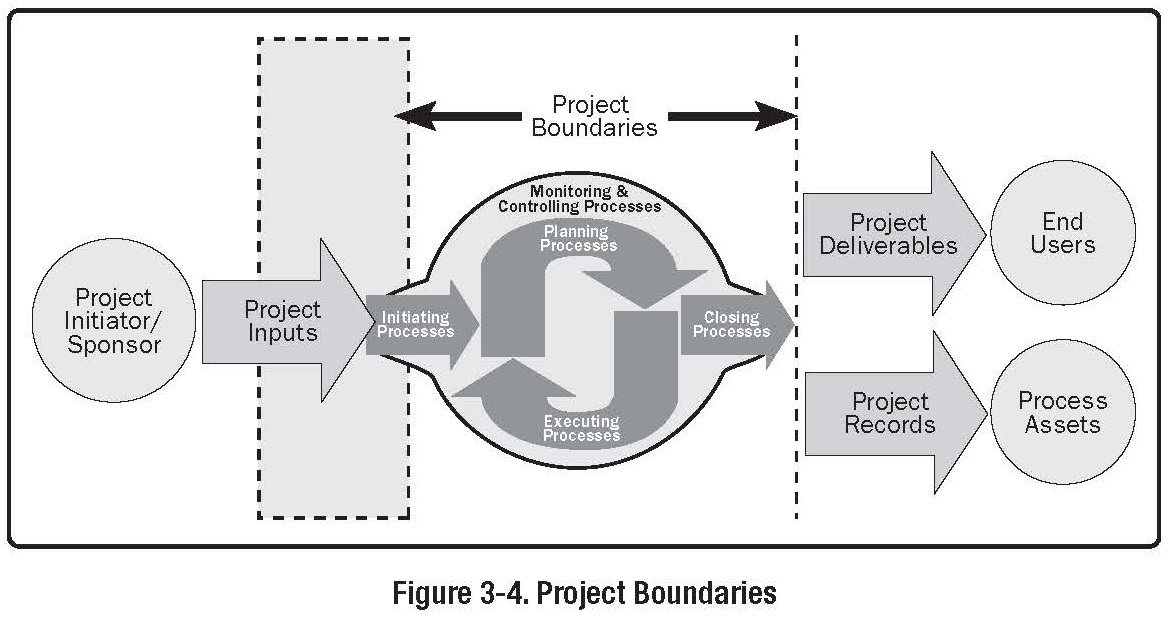
\includegraphics[width = 8cm]{images/Fig3-4.jpg}
 	\label{fig:3-4}
 \end{figure}
\end{frame}
\begin{center}\line(1,0){250}\end{center}



\begin{frame}
\frametitle{Initiating Process Group}
 \begin{figure}
 	\centering
 		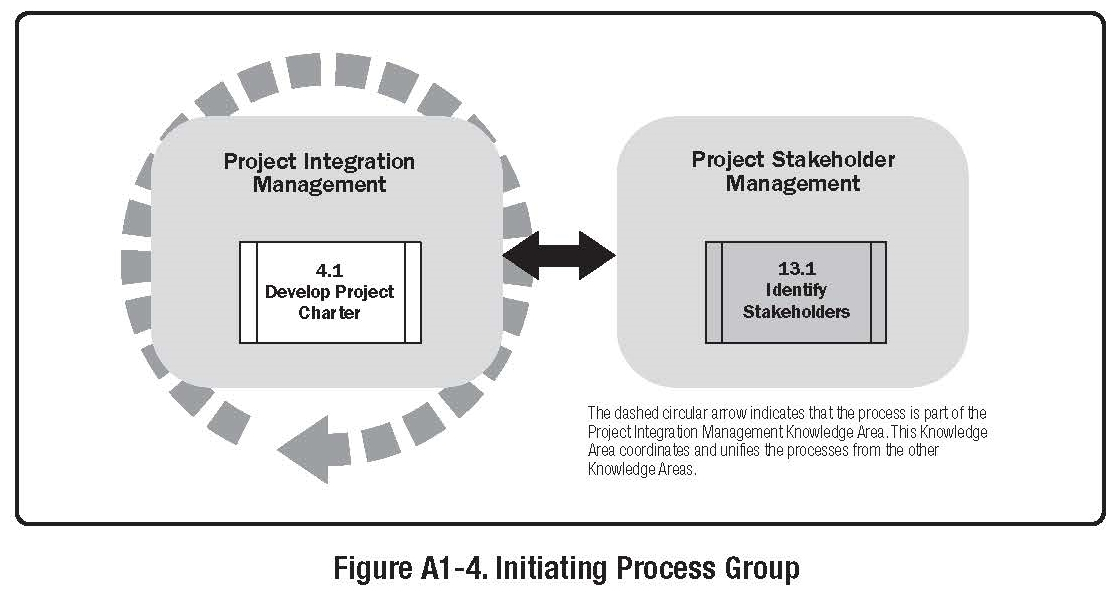
\includegraphics[width = 8cm]{images/FigA1-4.jpg}
 	\label{fig:1-4}
 \end{figure}
\end{frame}
\begin{center}\line(1,0){250}\end{center}



\begin{frame}
\frametitle{Initiating Process Group}
\begin{itemize}
	\item This is the formal commencement of the Project
	\item Used to validate the assumptions, decisions and constraints previously made and identified (Kill Point?)
	\item Project Manager is usually appointed at this stage
\end{itemize}
\end{frame}
\begin{center}\line(1,0){250}\end{center}



\begin{frame}
\frametitle{Initiating Process Group}
\begin{figure}
	\centering
		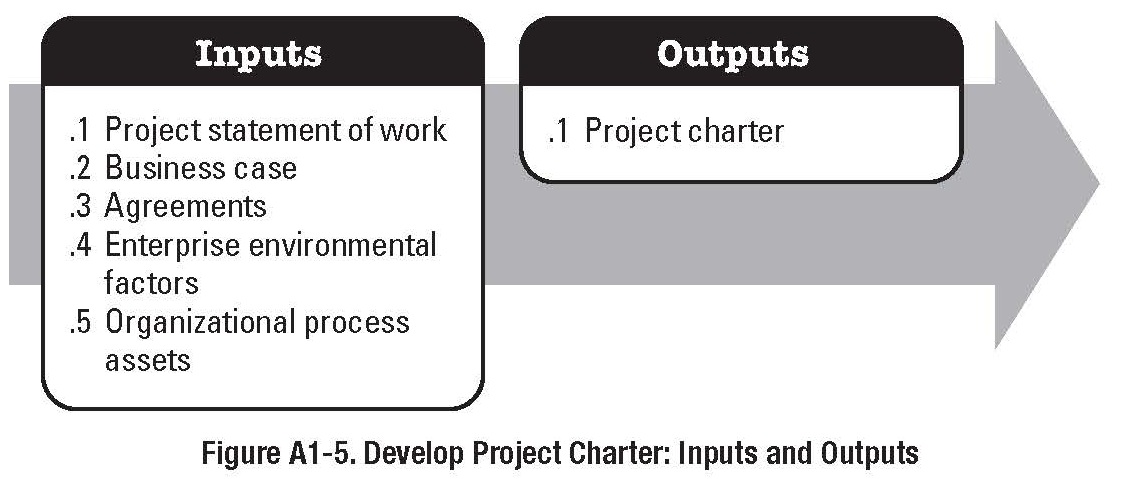
\includegraphics[width = 6cm]{images/FigA1-5.jpg}
	\label{fig:A1-5}
\end{figure} 
\begin{itemize}
	\item Project Charter developed during this process includes information identified in the previous stages
	\item This Project Charter requires approval and authorisation.
	\item Approval and Funding are external to the PM Team
\end{itemize}
\end{frame}
\begin{center}\line(1,0){250}\end{center}



\begin{frame}
\frametitle{Initiating Process Group}
\begin{figure}
	\centering
		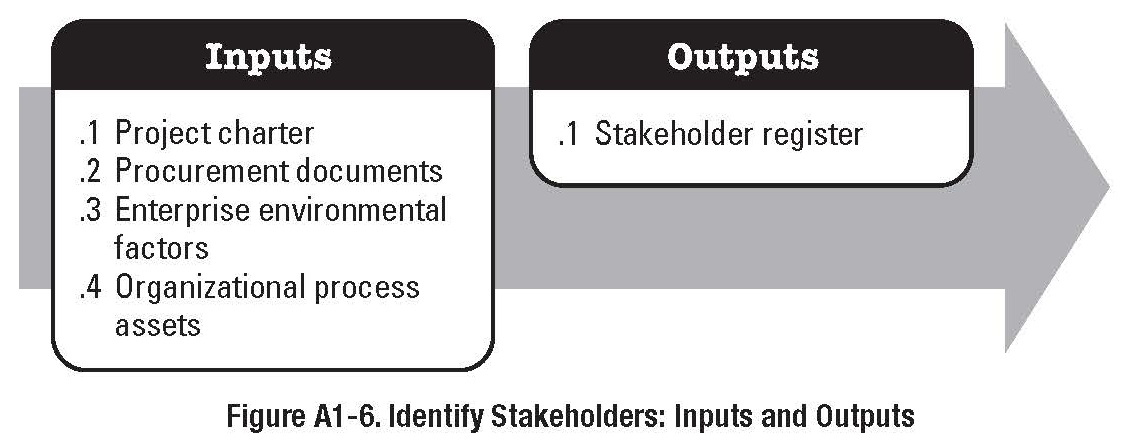
\includegraphics[width = 6cm]{images/FigA1-6.jpg}
	\label{fig:A1-6}
\end{figure} 
Identify Stakeholders is the process of identifying all people or organisations impacted by the project and documenting relevant information regarding their interests, involvement, and impact on project success.
\end{frame}
\begin{center}\line(1,0){250}\end{center}



\begin{frame}
\frametitle{Planning Process Group}
 \begin{figure}
 	\centering
 		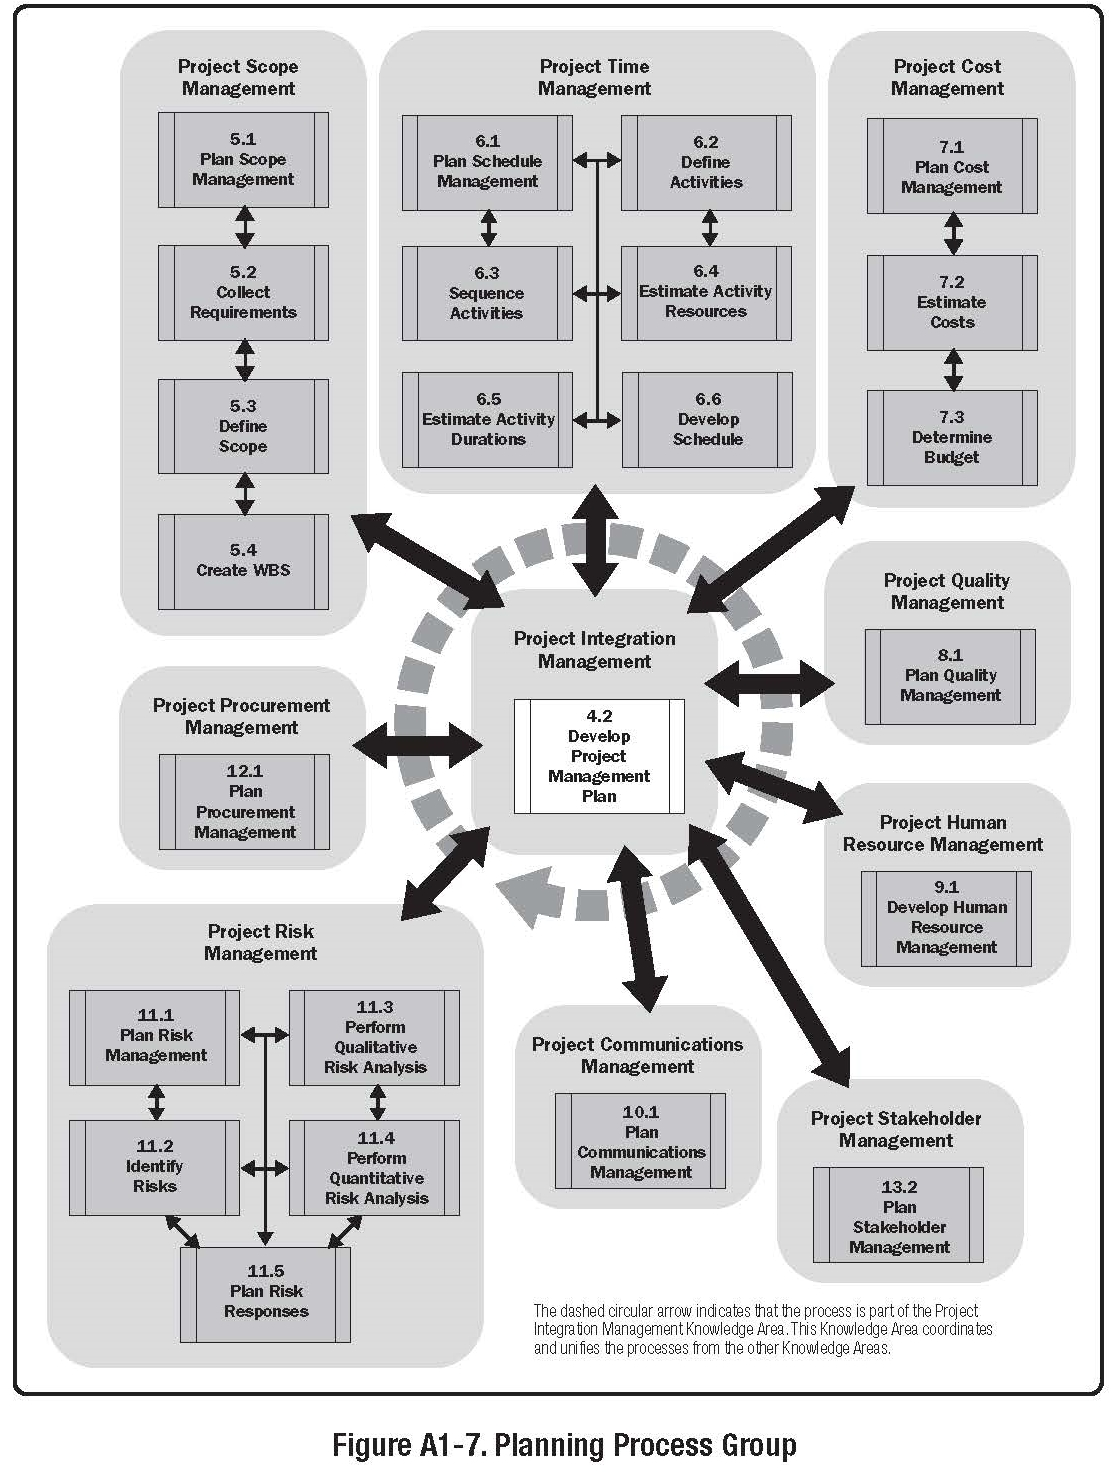
\includegraphics[width = 5cm]{images/FigA1-7.jpg}
 	\label{fig:A1-7}
 \end{figure}
\end{frame}
\begin{center}\line(1,0){250}\end{center}



\begin{frame}
\frametitle{Planning Process Group}
Thought by many to be the most important\\
\begin{itemize}
	\item it is vital, but pointless if not integrated into all other aspects of Project Management Process Groups
\end{itemize}
PP Group is used to develop the PM Plan\\
These processes identify, define and mature the project scope, cost, and schedule\\
The PP Group should involve all relevant stakeholders - Trilogy (2003) Project failed in this respect\\
It is an iterative process\\
\begin{itemize}
	\item For instance a schedule risk may not be identified until `activity duration estimating' has been completed
\end{itemize}
Cannot continue indefinitely; the executing organisation should set a date for completion, dependant on the nature of the project. (General Management Issue)\\
\end{frame}
\begin{center}\line(1,0){250}\end{center}



\begin{frame}
\frametitle{Planning Process Group \hfill Define Scope  }
 \begin{figure}
 	\centering
 		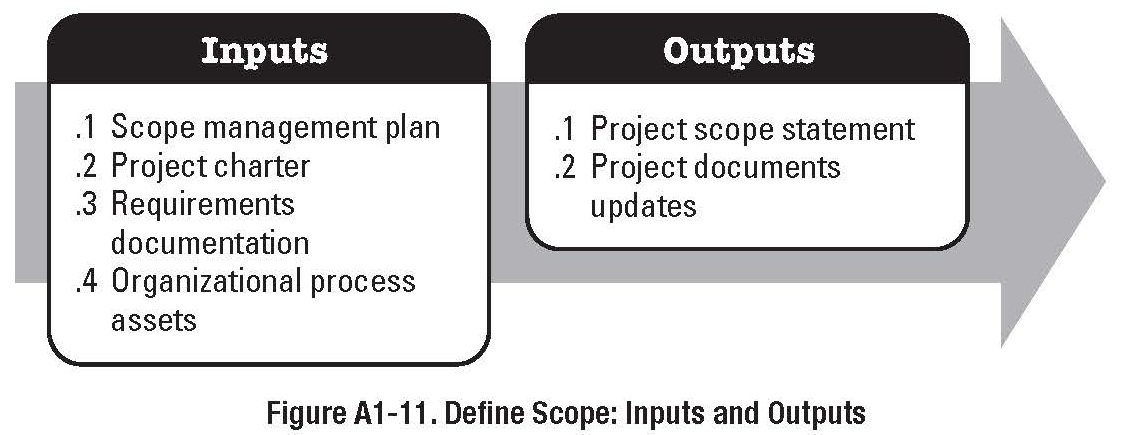
\includegraphics[width = 8cm]{images/FigA1-11.jpg}
 	\label{fig:A1-11}
 \end{figure} 
\end{frame}
\begin{center}\line(1,0){250}\end{center}



\begin{frame}
\frametitle{Planning Process Group \hfill Create WBS}
 \begin{figure}
 	\centering
 		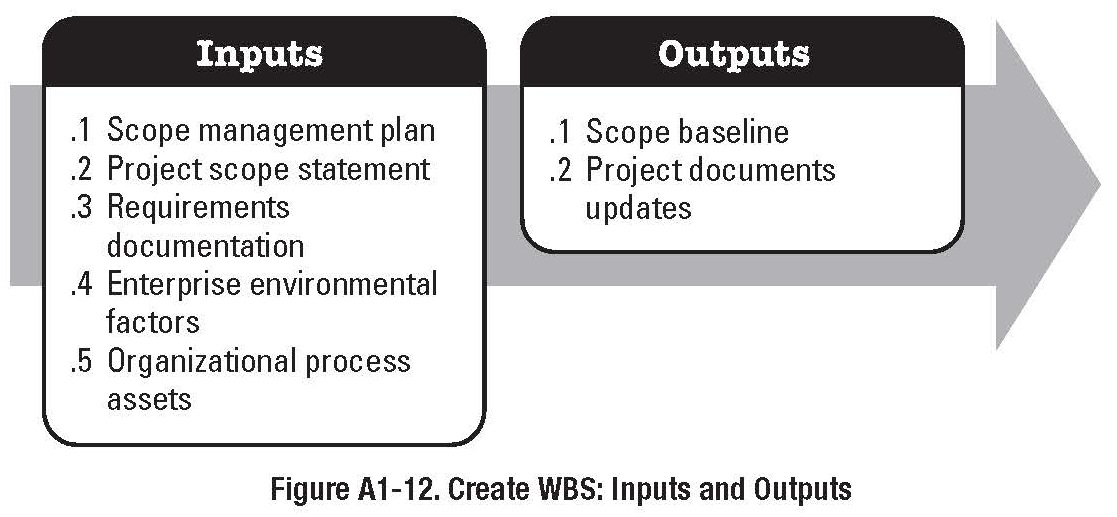
\includegraphics[width = 8cm]{images/FigA1-12.jpg}
 	\label{fig:A1-12}
 \end{figure}
\end{frame}
\begin{center}\line(1,0){250}\end{center}



\begin{frame}
\frametitle{Planning Process Group \hfill Activity Sequencing}
 \begin{figure}
 	\centering
 		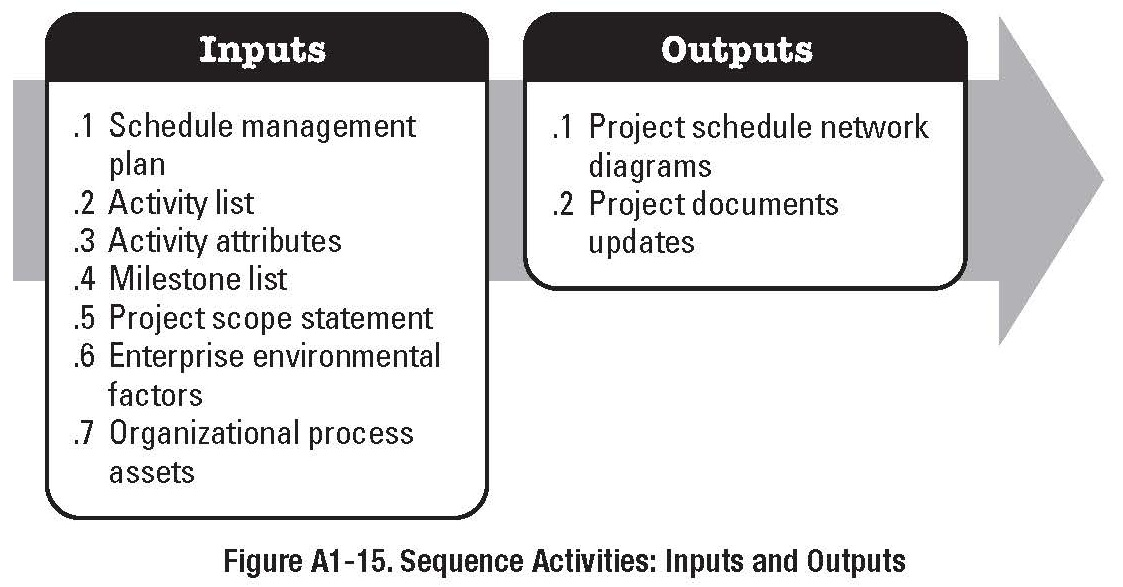
\includegraphics[width = 8cm]{images/FigA1-15.jpg}
 	\label{fig:A1-15}
 \end{figure}
\end{frame}
\begin{center}\line(1,0){250}\end{center}



\begin{frame}
\frametitle{Planning Process Group \hfill Cost Budgeting}
 \begin{figure}
 	\centering
 		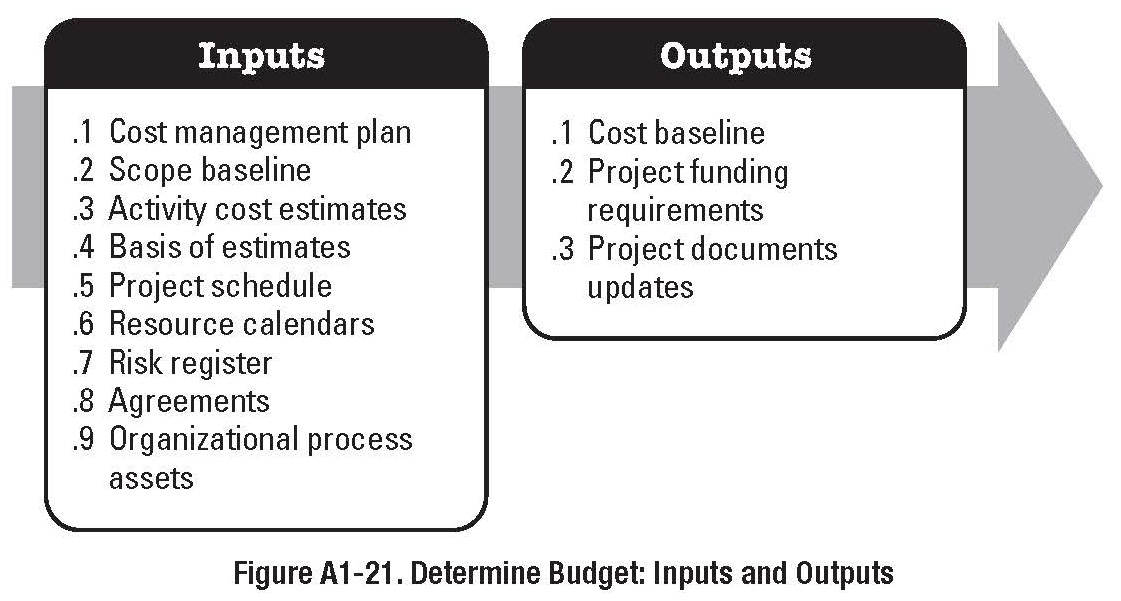
\includegraphics[width = 8cm]{images/FigA1-21.jpg}
 	\label{fig:A1-21}
 \end{figure}
\end{frame}
\begin{center}\line(1,0){250}\end{center}



\begin{frame}
\frametitle{Planning Process Group \hfill Risk Identification}
 \begin{figure}
 	\centering
 		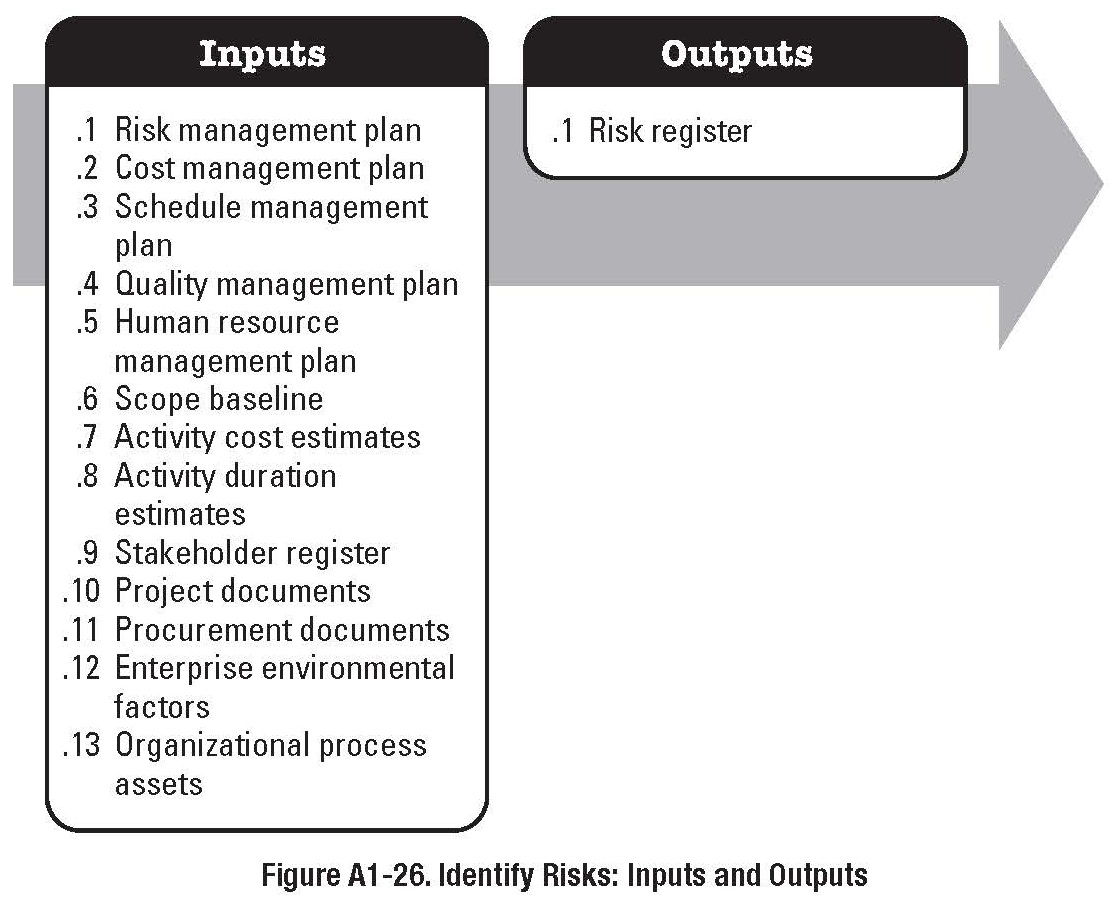
\includegraphics[width = 8cm]{images/FigA1-26.jpg}
 	\label{fig:A1-26}
 \end{figure}
\end{frame}
\begin{center}\line(1,0){250}\end{center}



\begin{frame}
\frametitle{Planning Process Group \hfill Quantitative Risk Analysis}
 \begin{figure}
 	\centering
 		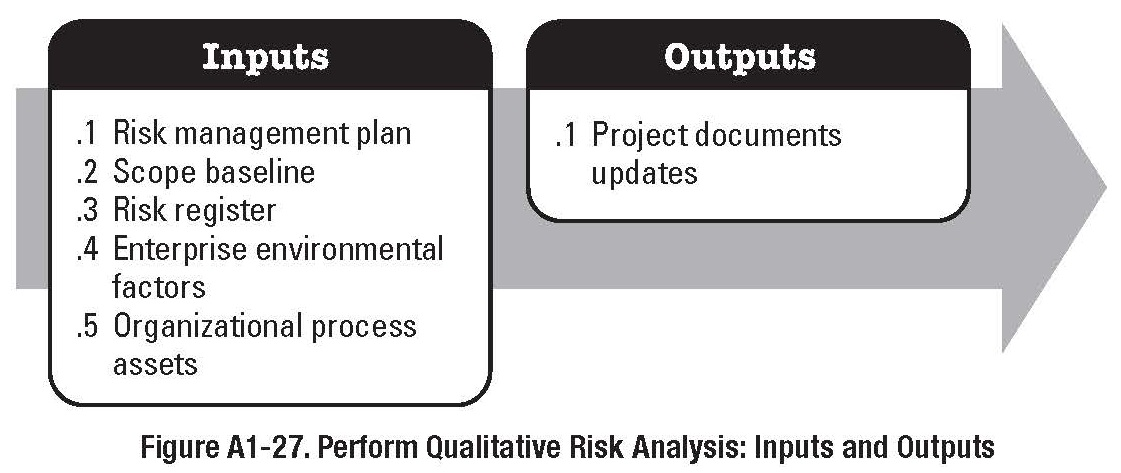
\includegraphics[width = 8cm]{images/FigA1-27.jpg}
 	\label{fig:A1-27}
 \end{figure}
\end{frame}
\begin{center}\line(1,0){250}\end{center}



\begin{frame}
\frametitle{Executing Process Group}
 \begin{figure}
 	\centering
 		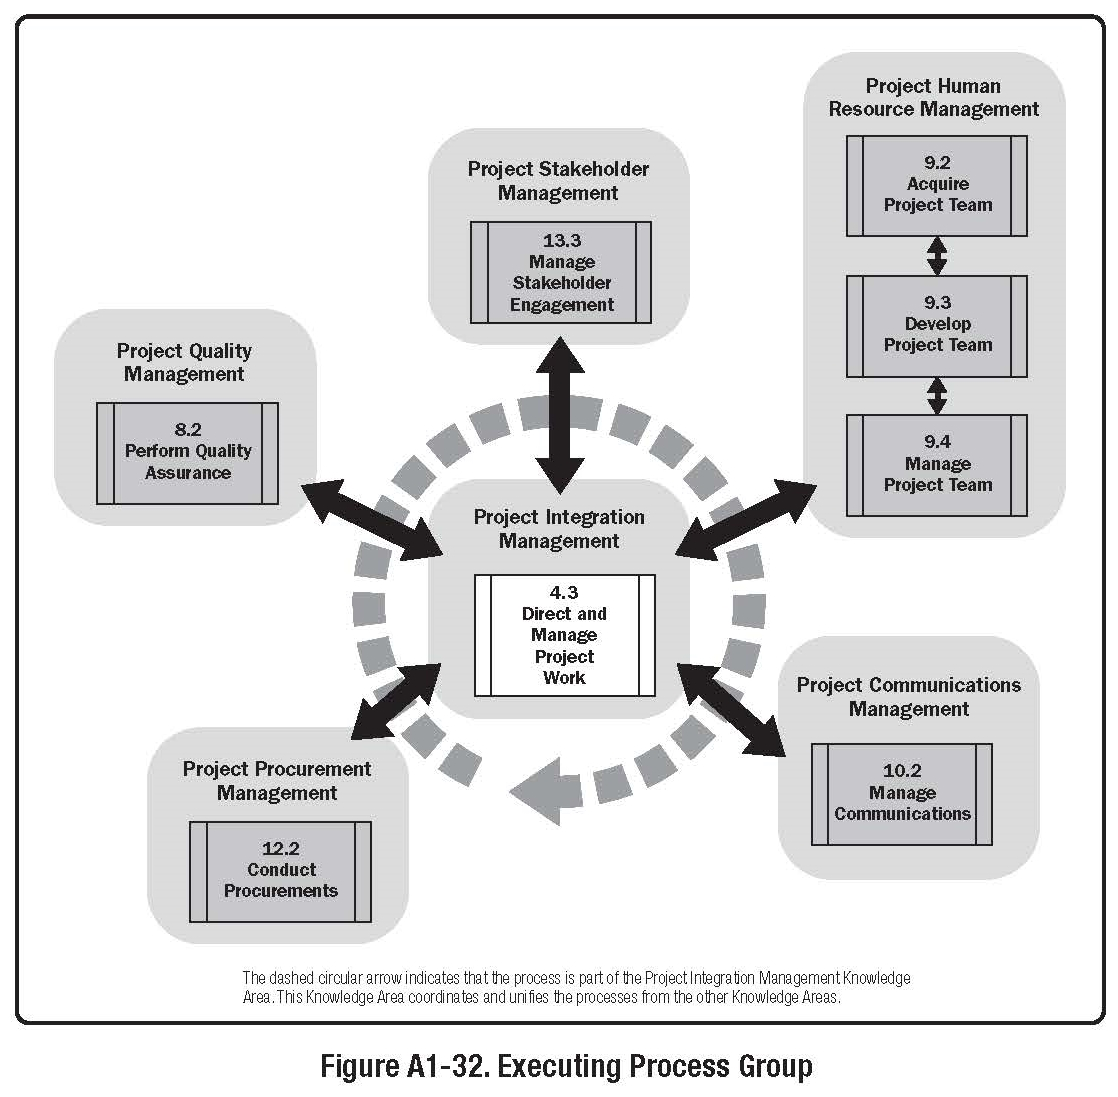
\includegraphics[width = 6cm]{images/FigA1-32.jpg}
 	\label{fig:A1-32}
 \end{figure}
\end{frame}
\begin{center}\line(1,0){250}\end{center}



\begin{frame}
\frametitle{Executing Process Group}
\begin{itemize}
	\item This process group consists of processes used to complete the work defined in the project management plan.
	\item The Executing P.G. involves coordination of people and resources, as well as integrating and performing the activities in accordance with the PM Plan
	\item This process group also addresses issues of Scope and change control.
	\item Normally, execution will cause changes to planning; identify previously unknown risks; etc.  Not all changes effect the PM Plan, but usually require analysis
	\item The vast majority of the Project Budget is expended in performing the Executing Process Group. 
\end{itemize}
\end{frame}
\begin{center}\line(1,0){250}\end{center}



\begin{frame}
\frametitle{Monitoring \& Controlling Process Group}
 \begin{figure}
 	\centering
 		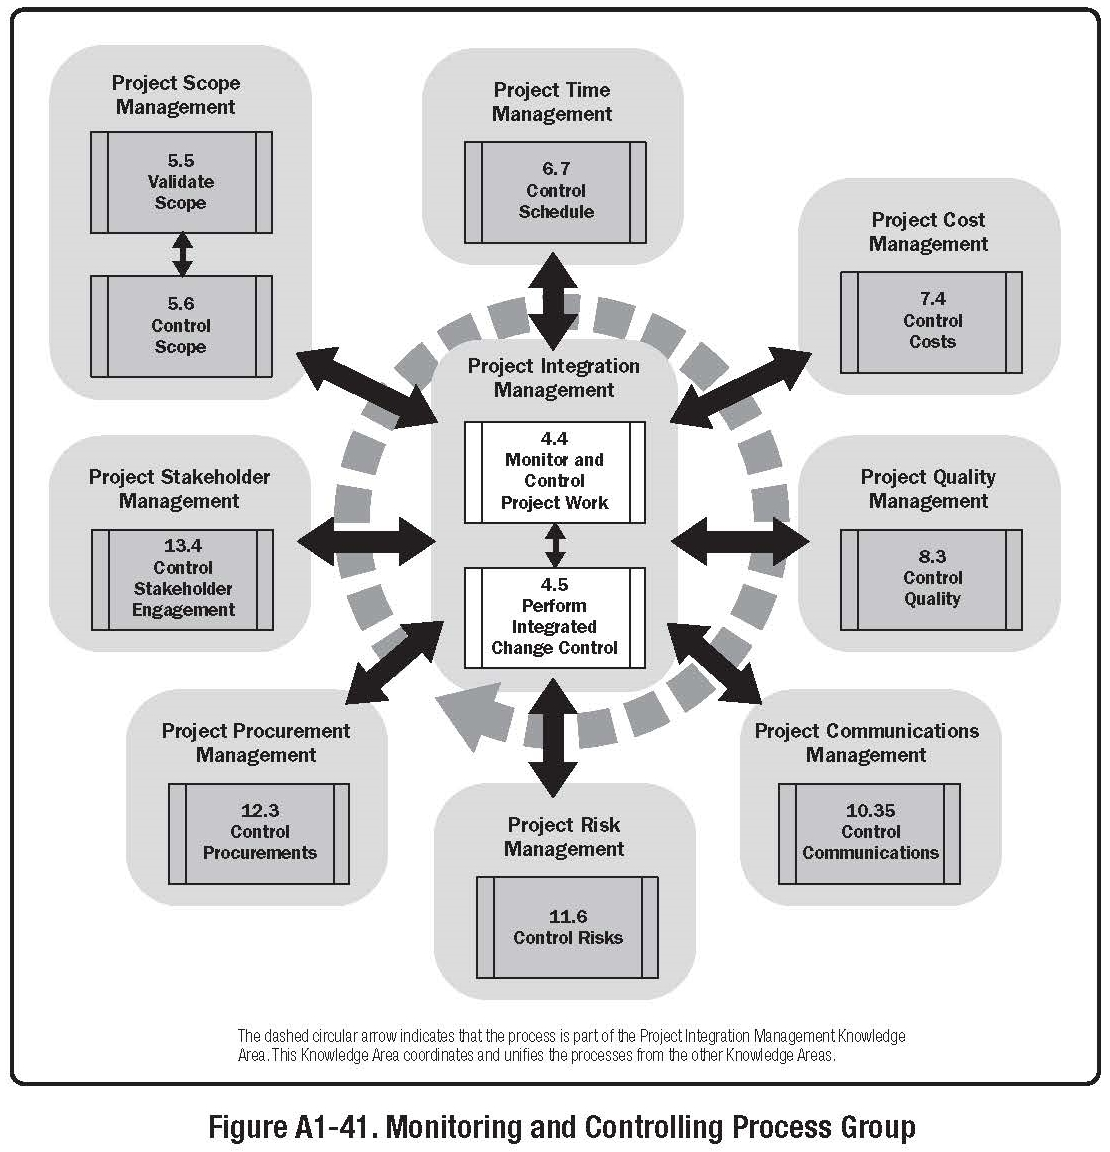
\includegraphics[width = 6cm]{images/FigA1-41.jpg}
 	\label{fig:A1-41}
 \end{figure}
\end{frame}
\begin{center}\line(1,0){250}\end{center}



\begin{frame}
\frametitle{Monitoring \& Controlling Process Group}
\begin{itemize}
	\item The M\&C process group consists processes used to \textbf{observe} project execution.
\begin{itemize}
	\item Used to identify potential problems, corrective actions, and control project execution.
\end{itemize}
	\item The output of these processes are compared with the project plan
	\item Also includes Change Control, Preventative Actions, 
	\item It is a continuous process, providing an insight into the status of the entire project at any given time
	\item This information may necessitate the modification of the overall project plan.
\end{itemize}
\end{frame}
\begin{center}\line(1,0){250}\end{center}



\begin{frame}
\frametitle{Closing Process Group}
 \begin{figure}
 	\centering
 		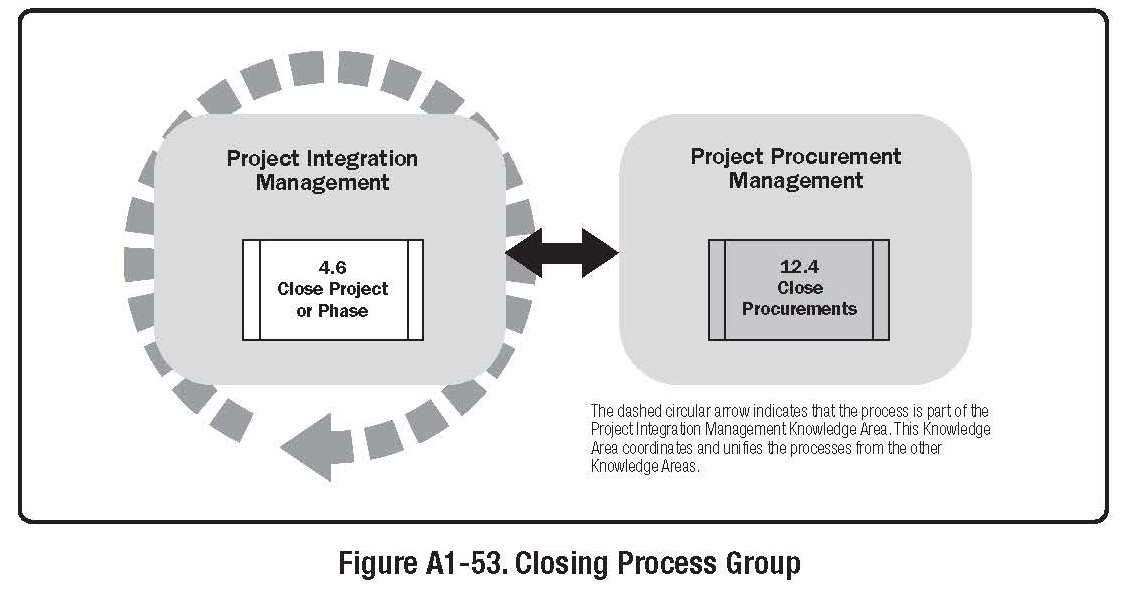
\includegraphics[width = 8cm]{images/FigA1-53.jpg}
 	\label{fig:A1-53}
 \end{figure}
\end{frame}
\begin{center}\line(1,0){250}\end{center}



\begin{frame}
\frametitle{Closing Process Group}
\begin{itemize}
	\item The closing process group includes processes used to \textbf{\textit{formally}} terminate all activities of a project or project phase
	\item When completed, this process group verifies that all processes defined within the other process groups are completed, and formally establishes that the project or project phase is finished.
\end{itemize}
\end{frame}
\begin{center}\line(1,0){250}\end{center}



\begin{frame}
\frametitle{Process Interactions}
 \begin{figure}
 	\centering
 		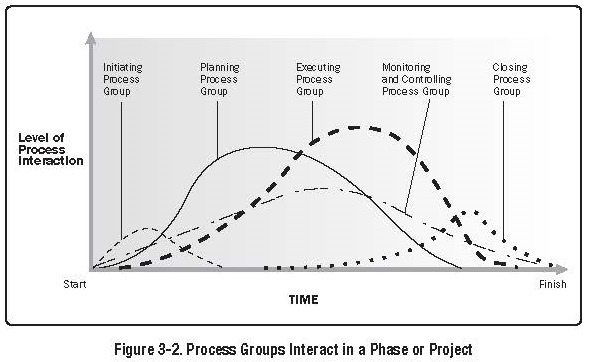
\includegraphics[width = 9cm]{images/Fig3-2.jpg}
 	\label{fig:3-2}
 \end{figure}
\end{frame}
\begin{center}\line(1,0){250}\end{center}



\begin{frame}
\frametitle{Process Interactions}
\begin{itemize}
	\item The Process Groups are linked; they are not independent of each other.\\
	\item Generally the output of one process becomes the input of another process\\
	\item Processes Groups are seldom, if ever, discrete events; often overlap with other groups.\\
	\item The level of interaction generally depends on how far the project has progressed.\\
	\item If a project is split into formal phases, these interactions may cross over project phases. \\ 
		\begin{itemize}
			\item Tends to present difficulties when it does. 
		\end{itemize}
\end{itemize}
\end{frame}
\begin{center}\line(1,0){250}\end{center}



\begin{frame}
\frametitle{Process Interactions}
\begin{itemize}
	\item Not all processes are required on all projects; not all process interactions are present on all projects\\
	\item The PM team must decide which processes to run and how to run them. 
		\begin{itemize}
			\item (may be governed/dictated by PMO, or Company Protocol) 
		\end{itemize}
\end{itemize}
\end{frame}
\begin{center}\line(1,0){250}\end{center}



\begin{frame}
\frametitle{Single Phase Project}
 \begin{figure}
 	\centering
 		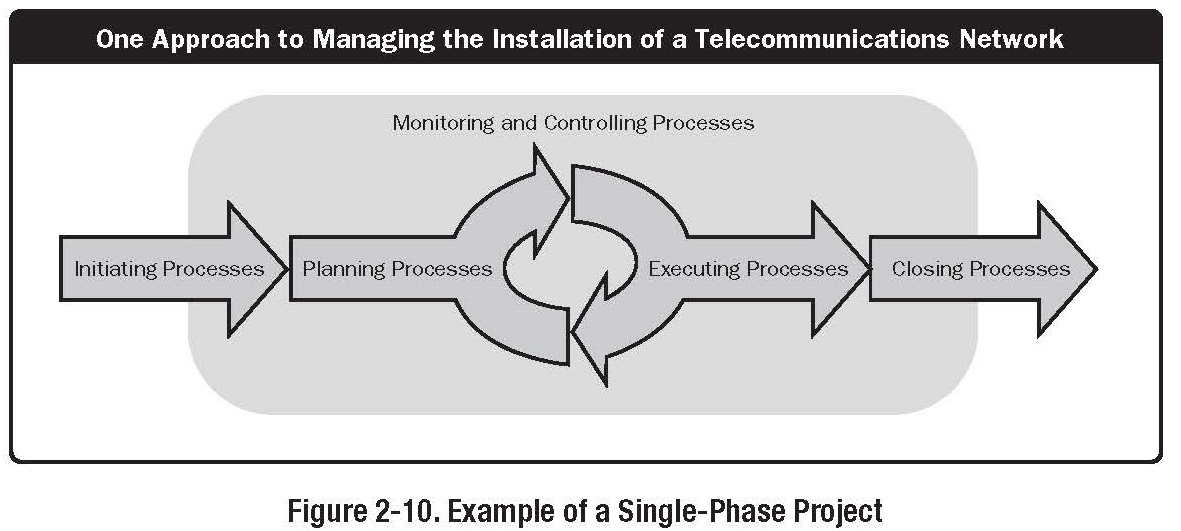
\includegraphics[width = 10cm]{images/Fig2-10.jpg}
 	\label{fig:2-10}
 \end{figure}
\end{frame}
\begin{center}\line(1,0){250}\end{center}



\begin{frame}
\frametitle{Multiphase project}
 \begin{figure}
 	\centering
 		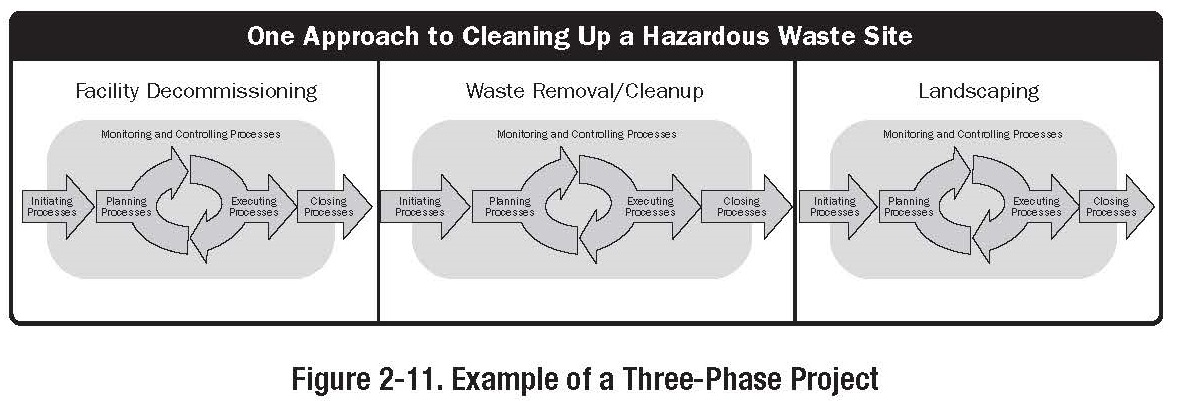
\includegraphics[width = 10cm]{images/Fig2-11.jpg}
 	\label{fig:2-11}
 \end{figure}
\end{frame}
\begin{center}\line(1,0){250}\end{center}



\begin{frame}
\frametitle{Overlapping Phases}
 \begin{figure}
 	\centering
 		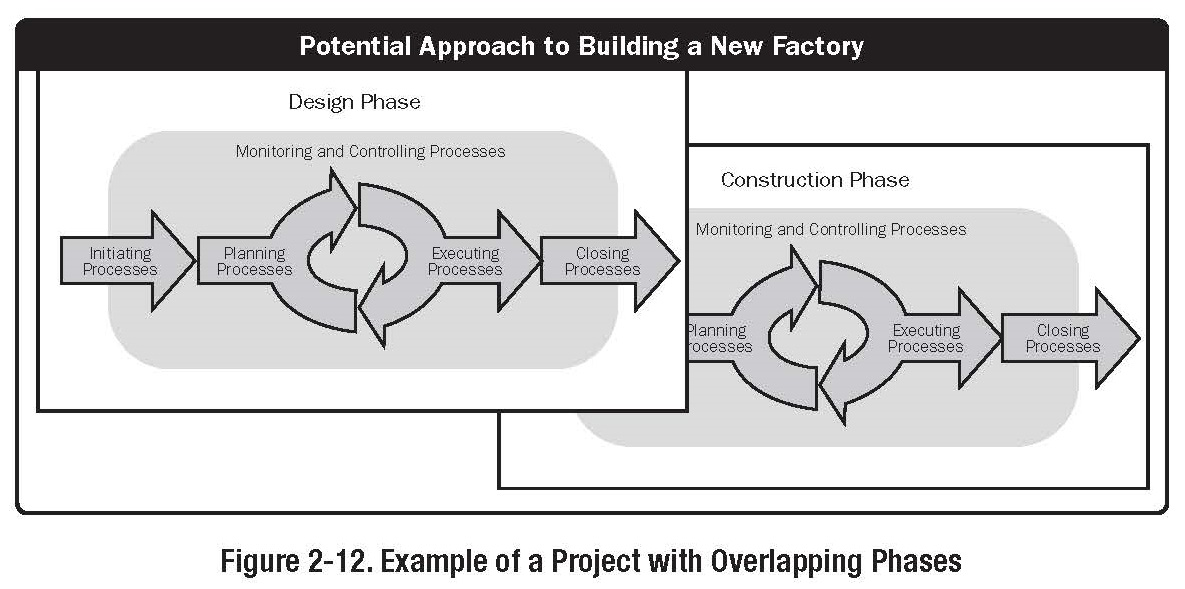
\includegraphics[width = 10cm]{images/Fig2-12.jpg}
 	\label{fig:2-12}
 \end{figure}
\end{frame}
\begin{center}\line(1,0){250}\end{center}
\begin{frame}
\frametitle{Project Management Process Mapping}
\begin{columns}
		\begin{column}{0.6\textwidth}		
			\begin{itemize}
				\item The 5 Process Groups contain a total of 47 Project Management Processes.\\
				\item Each Process is shown in the Group in which most of its activity takes place.\\
					\begin{itemize}
						\item i.e if a process is undertaken during `planning' is revisited during `execution', then it is the same process, not a new one
						\item \textbf{Remember: Not all processes are required on every project}
					\end{itemize}
			\end{itemize}
		\end{column}	
			
		\begin{column}{0.4\textwidth}	
			\begin{figure}
				\centering
					\includegraphics[width = 4cm]{images/tbl3-1.jpg}
				\label{tbl:3-1}
			\end{figure}
		\end{column}
\end{columns}

\end{frame}
\begin{center}\line(1,0){250}\end{center}



\begin{frame}
\frametitle{Project Management Process Mapping}
 \begin{figure}
 	\centering
 		\includegraphics[width = 7cm]{images/tbl3-1a.jpg}
 	\label{tbl:3-1a}
 \end{figure}
\end{frame}
\begin{center}\line(1,0){250}\end{center}



\begin{frame}
\frametitle{Project Management Process Mapping}
 \begin{figure}
 	\centering
 		\includegraphics[width = 7cm]{images/tbl3-1b.jpg}
 	\label{tbl3-1b}
 \end{figure}
\end{frame}
\begin{center}\line(1,0){250}\end{center}

\end{document}
